\documentclass [a4paper, 11pt, titlepage] {article}

\usepackage[ansinew]{inputenc}
\usepackage[english]{babel}
\usepackage{amsmath,amssymb,amsfonts}
\usepackage{verbatim}
\usepackage{graphicx}
\usepackage{fancyhdr}
\usepackage{lscape}
\usepackage[pdftex,bookmarksnumbered,colorlinks,backref, bookmarks, breaklinks, linktocpage]{hyperref}
\usepackage{subfig}
\usepackage{listings}
\lstset{
  language=ruby, %The programminglanguage to be used
  showspaces=false, %Leaves spaces blank
  showstringspaces=false, %Leaves spaces in strings blank
  breaklines=true, %Break lines that are too long
  basicstyle=\tiny, %The text style and size of the code
  extendedchars=true, %Includes danish characters
  numbers = left, %Shows linenumbers
  stepnumber = 1, %The interval with which linenumbers are displayed
  numberstyle=\tiny %The label size
}

\frenchspacing \setlength{\parindent}{0pt}
\setlength{\parskip}{1ex plus 0.5ex minus 0.2ex}

\addtolength{\textwidth}{1cm}
\addtolength{\textheight}{1cm}
\setlength{\parindent}{0pt} % for adjusting indentation

\hyphenation{desirable finally sta-ti-sti-cal-ly basic tailored}
\date{A date}

\newcommand{\singleimwidth}{0.9\textwidth}
\newcommand{\doubleimwidth}{0.5\textwidth}

%BEGIN Changing sizes of captions:

% Different font in captions
\newcommand{\captionfonts}{\footnotesize}
\newcommand{\mycomment}[1]{
\begin{center}
\fbox{
\begin{minipage}{0.8\textwidth}
\it
#1
\end{minipage}
}
\end{center}
}

\begin{document}

\setlength{\parindent}{4mm}

\begin{titlepage}
  \begin{center}
    \vspace*{\stretch{1}}
    \noindent\rule{\linewidth}{1mm}\\[4mm]
      {\sffamily\bfseries \Huge Intelligent Traffic Light Management}\\[1mm]
      {\sffamily\bfseries \Large Arterial Simulation \& Optimization}\\[0mm]
    \noindent\rule{\linewidth}{1mm}\\[30mm]
    \large $\overline{\textrm{ Andreas Warberg, 030447 }}$

    \vspace*{\stretch{3}}

    \large \today \\[6mm]
Supervisors: \\
Ren\'{e} Munk J�rgensen, DTU Transport \& \\ 
Jesper Larsen, DTU Management\\[3mm]
\textbf{Technical University of Denmark}
  \end{center}
\end{titlepage}

\newpage
\section*{Abstract}
The signal controllers of heavy-traffic arteries are subject to optimization to best accomodate the movement of the large traffic volumes.
The DOGS system for arterial optimization was tested in the Vissim microsimulator for a section of the Danish ringroad 3. Tests show that DOGS, while providing improved conditions for arterial traffic, can be further improved by selecting an offset for each DOGS level, rather than remaining at the same offset regardless of the currently selected cycle time. For finding such offsets for the comparison a simulated annealing algorithm was implemented to solve the coordination problem ie. finding offsets.

Keywords: \textbf{traffic signal settings}, \textbf{traffic optimization}, \textbf{traffic artery}
\newpage
\pagenumbering{roman}
\tableofcontents
\newpage
\pagenumbering{arabic}

\section{Introduction}

Road traffic is an essential part of modern society and has put a high
demand on road networks. Figures from a recent study from the Danish
ministry of transport \cite{47} shows traffic has increased by 50\%
since the 80's and that cars and busses are responsible for more than
90\% of all person transport in Denmark (totalling 68 milliom
kilometers).

Traffic network congestion causes delays which adds substantial costs
to the society and businesses on a daily basis and also increases
emissions and the risk of accidents. In the beforementioned study it
is reported that in 2002 people where spending 100,000 hours in total
in queue in the Greather Copenhagen road infrastructure, this
corresponds to an economic loss of more than 750 million Euros.  

To alleviate congestion, public transport can be improved or the
infrastructure can be expanded. In urban areas, the latter is often
impossible due to residential areas adjacent to the existing roads.
A more subtle way to improve the network performance is to make better
use of the existing roads, which can be done by proper setting of
traffic signal parameters.

It is estimated that the proper use of intelligent traffic systems
including intelligent traffic signals can increase the capacity of the
road network in the Greater Copenhagen area by 5 to 10\%.

Traffic signals are employed in urban areas in order to control
traffic flows and avoid collisions by fairly distributing the
right-of-way for adjoining road segments and to ensure a smooth flow
of traffic. If not set appropriately traffic signals may seriously
affect the traffic flow through the road network and so great care
should be taken when choosing the parameters for an intersection.

The literature has many suggestions for the intelligent setting of
traffic signals, ranging from purely statistically based methods
developed in the early 60's over actuated traffic signals to highly
adaptive and cooperative methods, which can be realized using actual
flow information supplied by traffic detectors. This paper gives a
survey of the literature with special emphasis on adaptive methods,
which attempts to coordinate traffic signals in larger networks so as
to optimize some network-wide performance index such as number of
stops or delay.

The paper is structured as follows. XXX Oversigt skal skrive naar
resten er paa plads XXX. Finally in section \ref{sec:conclusion} we
summarize the findings and come with recommendations for future works.


\newpage

\section{Signal Control Systems}
\label{systems}
The systems that mandate road use by signal controllers can roughly be divided into two major types: adaptive and non-adaptive. Within each type the systems are specialized with respect to the number of signal controllers the system governs and the network layout, when more than one intersection is under signal control. 

The general traffic light management system manage the settings of signal controllers in a grid of connected roads and the optimization problem must respect all traffic flows between each input and output. A special case is the \textit{artery} where a single one-way or bidirectional traffic flow dominates the total demand of the network.

This section introduces briefly the major trends in these two systems to outline the setting in which DOGS is used.

\subsection{Traditional signal control}

The traditional systems, which are also the simplest, operate on the basis of signal plans, such as the ones seen in appendix \ref{app:signalplans}. For isolated intersections, there is a choice between pretimed and traffic actuated control strategies. Pretimed control involves the use of static signal plans for phase sequences, cycle time and green times according to the time of day. Traffic actuated signals are usually flexible versions of the static signal plans, allowing the green time of stages to be extended, up to some maximum when vehicles are detected.

When more than one signal controller is under system control the signal plans are based on a common cycle time and the signal controllers are adjusted relative to each other by choosing an offset, for each signal controller, which provides good coordination. Traffic actuated signals cannot cooperate with other signal controllers in an artery since they operate on a variable cycle time depending on the amount of time each stage was extended.

Pretimed control is based on the assumption that demand is fairly stable within certain divisions of time eg. morning, midday and evening or workday / weekend. For instance, in the morning (7.00 to 9.00) and afternoon (15.00 to 17.00) the traffic is usually heavier than during the day or night due to  commuter traffic.

Tools such as TRANSYT are used to generate static signal plans and offsets given historical traffic data.

\subsection{Adaptive signal control}
Adaptive signal control strategies may be based on historical data as well, but differ from schemes using static signal plans by actively monitoring current traffic conditions and make adjustments accordingly.

The dynamic aspects of traffic become obvious when considering the things that affect it:

\begin{itemize}
\item Events: football games, lane closures due to VIP transport etc. will cause a focusing of traffic in certain areas
\item Weather: warm weather will cause more traffic going out of the city while winter and snow causes reduced speeds but potentially also fewer vehicles on the road
\item Accidents: traffic is diverted onto alternative routes
\end{itemize}

It is near impossible to take into account such phenomenon when designing pretimed signal plans. In fact traffic engineers will attempt to capture the least "eventful" (neutral) dataset possible when designing such plans to accomodate the most common traffic situation.

Adaptive signal control systems adjust signal controllers in an arterial or network to coordinate intersections so as to optimize some performance index eg. average delay or number of stops (or a combination) but also to reduce the need for constant supervision and tuning of signal timing plans, which is necessary for pretimed control. That said, an adaptive system will also need supervision, but at least they are designed to be able to make adjustments autonomously, such as redistributing green time from one direction to another, when traffic changes.

To achieve optimum combined performance, adaptive systems dynamically adjust parameters such as cycle times, phase sequences and green times according to detected as well as predicted traffic thereby reacting to those dynamic aspects of traffic, which cannot be captured by the pretimed signal plans. Systems like the phase-by-phase system in the article \cite{phase_by_phase}, RHODES \cite{rhodes}, OPAC \cite{opac} and SCOOT \cite{scoot} even skip or work around the conventional periodic scheme based on a common cycle time and make direct assignments of phases and allow phases to be skipped, as discussed later in section \ref{phase_based}. 

The key to adaptive signals is reliable detection and short term prediction of traffic. Most of the adaptive systems I analysized in \cite{forprojekt} use historical input and current detector input to make short term predictions for what is going to happen eg. within the next minute, next 10 minutes and so forth.

While an isolated signal controller operated in a traffic actuated scheme can be thought of as a primitive type of adaptive signal, the main attraction with adaptive signals is when they can be set to work together. A good system will naturally cause green waves to appear and move the direction of the green waves along with changes in flow.

It is evident that the cycle time is crucial in optimization because, in case of a congested network, increasing the cycle time will cause increased capacity and - hopefully - increased throughput as well. Long cycle times lead to long phase durations, which allow a steady flow of vehicles to pass and minimizes lost and interphase time per time unit, but will also allow queues to grow larger until they can be emptied by the start of a green stage for the approach of the queue. Thus increasing the cycle time increases the capacity of the intersection. The exception is for left-turning traffic, which does not have a priority stage, here long cycle times will actually decrease capacity since only as many vehicles as will fit in the intersection may turn per cycle.

\newpage
\label{sec:dogs}

DOGS is an extension of the DOG system. The first 3 letters can be
directly translated from danish to \textit{dynamic optimization of
greens} and the appended S of the herein regarded system means
\textit{coordination}. Thus DOG is an traffic actuated optimizer for
single intersections, as described in section \ref{insec:actuated},
and DOGS add coordination. The DRD has implemented DOGS along several
arterials in Denmark.

DOGS is a criteria-based system which relies on a common cycle time
for coordination. The intended area of application is traffic signals
along arterials, which see a high fluctuation in demand.

The purpose of DOGS is to increase the capacity of the arterial in
high demand periods and revert to offline-optimized, pretimed plans in
low traffic situations. The capacity increase is realized by
increasing the common cycle time and allocate the extra green time per
cycle to the phases along the arterial. This will cause increased
delays for the minor roads, but may prevent queues from reaching the
previous intersection - or even prevent queues in cases of light
congestion.  DOGS is also capable of providing priority to buses by
extending the green time when buses are near an intersection.

At present the system must be tailored to the environment in which it
operates. For this reason the following sections will use the Herlev
area in Denmark as a reference area in order to explain certain
concepts. In Figure \ref{fig:dogs_herlev} is a layout of this network.

\begin{figure}[!ht]
\begin{center}
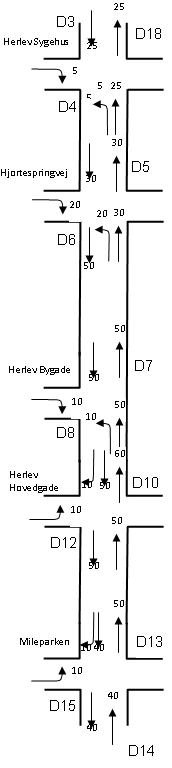
\includegraphics[scale=0.5,angle=90]{dogs_herlev.png} 
\end{center}
\caption{Layout of the partial O3 arterial in Herlev, which is under DOGS control. The arrows and numbers indicate flow direction and examples of typical vehicle count.}
\label{fig:dogs_herlev}
\end{figure}

\subsubsection*{Prediction}

DOGS is a purely traffic actuated system and no prediction is used
when the system is activated due to heavy traffic conditions.
In spite of the intended flexibility of the system this is a point
which puts high demand on the implementing traffic engineers since
traffic through the arterial must be assessed manually when the system
is put into production as well as during maintenance.

An alleviating point to the lack of prediction is the fact that the
current arterials under DOGS control are relatively small and static
predictions can be made by an experienced traffic
engineer. Furthermore, since DOGS only operate under high load
conditions, predictions become less valuable - or superfluous, even -
because all that can be said about the arterial in this case is that
it is heavily loaded with traffic.

\subsubsection*{Optimization}

Since DOGS only kicks in under congested or near-congested conditions
(for the Herlev area when the load exceeds 60\%) it is simple to
optimize the throughput since any increase in green time will just
allow more vehicles to pass (the phase is never emptied from
vehicles).

That DOGS only operates during high-congestion levels is an unusual trait for an adaptive system since they usually excel in optimization under \textit{normal} ie. uncongested load conditions (see the comparison of RHODES and a semi-actuated system in section \ref{sec:rhodes}). This can be explained from the lack of an explicitly defined objective function and optimization routine.

The objective is to keep the load degree (load/capacity) for the most heavily loaded intersection below 90\%.
To do this the common cycle time and green times are set according to the load level. The adjustments are made with a few seconds per cycle to avoid sudden, major changes in cycle time and temporary loss of coordination.

Coordination is achieved by running the signals on a common cycle time, but offsets are not adjusted when the common cycle time changes so this issue should receive further investigation.

A set of non-overlapping criteria are used to select a program with the appropiate capacity for the detected inflow. For a technical description of these criteria cf. \cite{forprojekt}

%% When naming the inflow detectors in the north- and south ends $DN$ and $DS$, respectively, the transition from pretimed control to adaptive control is decided by the constraint:
%% \begin{eqnarray*}
%% Intensity(DN) > I_{enable} & \vee & Intensity(DS) > I_{enable} \\
%% & or & \\
%% Load(DN) > L_{enable} & \vee & Load(DS) > L_{enable}
%% \end{eqnarray*}

%% For switching back to pretimed control this constraint must hold:
%% \begin{eqnarray*}
%% Intensity(DN) < I_{disable} & \wedge & Intensity(DS) < I_{disable} \\
%% & and & \\
%% Load(DN) < L_{disable} & \wedge & Load(DS) < L_{disable}
%% \end{eqnarray*}

%% To avoid hysteresis ie. constant enabling and disabling of dynamic control:
%% \begin{eqnarray}
%% I_{enable} - I_{disable} & \geq & I_{\varepsilon} \label{eqn:hysteresis_intensity} \\ 
%% L_{enable} - L_{disable} & \geq & L_{\varepsilon} \label{eqn:hysteresis_load} \\
%% I_{\varepsilon},L_{\varepsilon} & > & 0 \label{eqn:hysteresis_limits}
%% \label{eqn:hysteresis}
%% \end{eqnarray}

%% DOGS exhibits a dynamic behaviour because the permitted cycle time extensions are divided into \textit{programs} according to the intensity and load levels in the ends of the artery. These program constraints take a form which is similar to the enable- and disable constraints.

%% When deciding whether to remain in the current program, $i-1$, or switch to a program for higher demand, $i$, the following relation must be satisfied:

%% \begin{eqnarray*}
%% I_{enable,i+1} \geq & \max(Intensity(DN),Intensity(DS)) & > I_{enable,i} \\
%% & \vee & \\
%% L_{enable,i+1} \geq & \max(Load(DN),Load(DS))  & > L_{enable,i}
%% \end{eqnarray*}

%% The decision of switching from program $i$ to the program for lower demand, $i-1$, is determined by this relation:

%% \begin{eqnarray*}
%% I_{disable,i-1} \leq & \max(Intensity(DN),Intensity(DS)) & < I_{disable,i} \\
%% & \wedge & \\
%% L_{disable,i-1} \leq & \max(Load(DN),Load(DS))  & < L_{disable,i}
%% \end{eqnarray*}

%% In the DOGS controlled area in Herlev there are 8 different programs to choose from and the enable and disable thresholds for programs respect the ordering implicit in the above equations:

%% $$\lbrace I,L \rbrace_{enable,i+1} > \lbrace I,L \rbrace_{enable,i}$$
%% $$\lbrace I,L \rbrace_{disable,i-1} < \lbrace I,L \rbrace_{disable,i}$$

%% To avoid hysteresis between programs the same constraints (equations \ref{eqn:hysteresis_intensity}-\ref{eqn:hysteresis_limits}) as for switching between pretimed and dynamic control applies.

\subsubsection*{Evaluation}

Tests have shown that the system is indeed capable of increasing the
capacity, with reduced queue lengths as a result. When the arterial in
Herlev is at or above moderate load DOGS will increase the capacity by
15-25\% compared to the capacity if only the pretimed plans was in
use.

\newpage
\section{Simulation \& Vissim}
\label{simulation}
Traffic simulation is the emulation of traffic on a computer and it is done to gain insight in road user behaviour and observe various effects eg. what happens to the minor-road traffic when we increase the cycle time to 100 seconds.

A main issue of traffic signal optimization is that of how to evaluate solutions. Fitness determination of a set of signal parameters is a major issue, especially in metaheuristic search, which is prevalent in the litterature and in this project, that put "blind faith" in the evaluation procedure. This is to be understood such that metaheuristic search routines do not necessarily search the solution space in a manner in which each step a better solution is obtained, but rather by trial-and-error. 
Furthermore the metaheuristic must evaluate a certain amount of solutions before confidence in the final solution is established, thus each evaluation must be fast if the search is a part of an adaptive system, rather than an offline optimization that has no strict deadline.

Simulation handles the complexity issues of modelling the bilevel system of mutually responsive road user behaviour versus traffic signal settings and allows the optimization routine to rely on the simulation results as a black box for fitness evaluation. 

The primary use of simulators are for infrastructure expansions and testing various signal timing plans, of course. In traffic signal optimization they are almost always used to establish confidence in performance for some signal optimization procedure. This confidence comes from observing the actions of the system during the simulation but also by comparing aggregated fitness values with those coming from some other, well-known approach. In this regard the TRANSYT offline traffic signal optimization package is often used as a baseline. 

This form of testing favors quality of the simulation over execution speed, unlike search routines, which must have results quickly. 
In Table \ref{tab:convergespeed} are the names of three major simulators, which are used by traffic engineers to produce realistic traffic simulations. 
In Denmark the de-facto simulation tool for final testing of signal settings and infrastructure changes has become Vissim by PTV. For obtaining signal settings TRANSYT is highly regarded by DRD though the results will often be adjusted and confirmed in Vissim.

There are three types of simulators, the main difference being the level of detail in the underlying model. They are micro-, meso- and macrosimulators. Microsimulators model the behaviour of each vehicle and driver, mesosimulators regard the movements of platoons of vehicles and macrosimulators search for equilibriums between signal settings and road user response (route choice), considering origins (input links) and destinations (output links).

Independent on the detail level of the model a simulation must run until it is converged before the fitness can be determined. 

Previous studies (see \cite{corsimvstransyt}) have shown that the CORSIM microsimulator is superior to the mesoscopic simulator from the TRANSYT package when combined with a genetic algorithm, since the flow equations do not capture the dynamic aspects of traffic. But microsimulation is also slower to converge and thus evaluation of a solution will take longer. In a comparison study \cite{simcompare} Holst estimates the required relative simulation time in a large network, see Table \ref{tab:convergespeed}.

\begin{table}[ht]
\centering
\begin{tabular}{c|c|c}
\textbf{Vissim} & \textbf{Dynameq} & \textbf{Time Slice Assistant} \\
\textit{(micro)} & \textit{(meso)} & \textit{(macro)} \\ \hline
1000 & 100 & 1
\end{tabular}
\caption{Estimate of of relative required simulation time for convergence. Convergence of a Vissim simulation takes approximately 1000 times longer then the same simulation in TSA.}
\label{tab:convergespeed}
\end{table}

Microsimulation will not scale as well as meso- and macrosimulation since the number of vehicles in the network will grow in proportion with the total length of the roads. In mesosimulation the number of platoons need not grow as fast since some arteries traverse the entire network and a single platoon is regarded. The headway threshold for platoon definition could also be increased to compensate for the extra cars. Macrosimulators will scale in proportion with the size of the OD-matrices, which is the minimal level of detail and complexity for realistic results. 
Meso- and macro simulators, using deterministic principles, have another advantage since they can execute heuristic procedures to skip past much of the initial population of roads, which is mandatory in microsimulation when traffic begins to flow into the empty network. Since most simulations will be stopped whenever convergence is reached this is a very useful attribute.

Aside from the commercial simulator packages, such as the ones listed in Table \ref{tab:convergespeed}, there are several examples of researchers implementing their own simulation tools. Such tools are tightly coupled to the test network and the results are questionable thus it is important that the industry agrees upon a common simulation platform, but also that common standards are used \textit{within} the agreed upon tool. Such a project has recently been undertaken by DRD to improve the comparability of results from different consulting firms.

\subsection{Vissim}
\label{vissim}
Vissim provides a microscopic simulation of traffic in a network. In this context microscopic entails that each vehicle is individually modelled and, in a sense, Vissim takes the view of the users of the network.

\subsubsection{Network Elements}

Vissim is highly flexible with regards to network layout description and intersection turning movements can be fine-tuned almost to perfection, given enough time. The network design process is done using a GUI interface where links are joined using connectors.

Links are directed sections of road with $n>=1$ lanes. All lanes have the same direction as the link - the opposite direction is modelled using a parallel link.

Connectors are mostly relevant in intersections where they connect exactly two links, however the lanes connected within the links can be chosen freely.

Vissim maintains a \textit{.inp} file, which contains the most relevant informations necessary to run a simulation including information on links, connectors and routes. 

\subsubsection{Traffic input}
Vissim is capable of dynamic traffic assignment (DTA) as well as static input. DTA is a method by \cite{Wardrop} in which the traffic flow adapts to the capacity of the network due to a \textit{stochastic user equilibrium} (SUE). 

Vissim can perform this form of traffic input given zones, which are confined and non-overlapping areas of the network, and a matrix describing the relative traffic from each zone to each other zone.

In this project DTA was abandoned on recommendation from DTU Transport professor Otto Anker Nielsen due to the dynamic nature of the traffic signals since, in his experience, odd phenomenon may occur such as unpredictable gridlocks, when adjacent links are fully saturated.

Instead static input was chosen. In static input traffic enters on specific links and traverse the network until an exit link has been reached. Static input is used in combination with routing decisions, which are usually placed on the input links such that each vehicle entering will immediately be assigned a route through the network.

Due to the number of input links and the need to run simulations with various inputs it was decided to implement routines to automate link input definitions.

Since Vissim relies on a text format it is possible to generate strings, which can be inserted in the appropriate section of the \textit{.inp} file.

The format of a link input is:
\begin{verbatim}
INPUT <input_number>
      NAME "<input_description>" LABEL  0.00 0.00
      LINK <link_number> Q <link_contrib> COMPOSITION <comp>
      TIME FROM <t_begin> UNTIL <t_end>
\end{verbatim}

(Vehicles always arrive at the beginning of the link.)

Where the most important fields are the \textit{link\_number}, defining on which link the input occurs, the \textit{link\_contrib}, which is the input quantity in vehicles per hour and finally \textit{t\_begin} and \textit{t\_end} ie. the time period in which this traffic quantity must be generated.

The \textit{comp} variable defines the traffic composition used eg. cars, trucks, buses or a combination. It is possible, but not recommended, to defined multiple inputs on the same link for the same period of time. Since the traffic composition will remain fairly static it is more intuitive to define a single link input for a traffic composition, which defines relative proportions of each possible vehicle type.

\subsubsection{Routing decisions}
\label{routingdecisions}
As mentioned routing decisions are made for vehicles immediately after they enter the system. This is done by placing a route decision point somewhere on an input link and designate a number of exit links, which can be internal links also, so as to generate a set of routes, which can be chosen among from some distribution.

For arterial simulation a general assumption is that most traffic is throughgoing. However, it is unrealistic to omit routes, which are not straight through. As will be seen in the data analysis section (\ref{data}), there are special circumstances to be handled for the two areas being modelled and thus is necessary to provide detailed route choices.

There exist many routes even for small networks when routes are symmetric (albeit using different links). Routes can be designed using the GUI tool provided with Vissim, however since the number of routes that can be taken will grow exponentially in the number of exit links, it is unfeasible to use this approach - especially if different route choice distributions are to be tested. Therefore it was decided to design route generation in the Vissim format, in addition to the before mentioned link input generator.

A routing decisions and the corresponding choice set takes the format:

\begin{verbatim}
ROUTING_DECISION <number> NAME "<description>" LABEL  0.00 0.00
     LINK <origin_link> AT 50.000
     TIME FROM 0.0 UNTIL 99999.0
     NODE 0
      VEHICLE_CLASSES <composition>
     ROUTE     1  DESTINATION LINK <dest_link1>  AT   5.000
     FRACTION <fraction1>
     OVER <connector> <link> ... <connector>
     ROUTE     2  DESTINATION LINK <dest_link2>  AT   5.000
     FRACTION <fraction2>
     OVER <connector> <link> ... <connector>
\end{verbatim}

The \textit{origin\_link} denotes the position of the decision point. The line \textit{VEHICLE\_CLASS...} impose a limit of the vehicles, which are required to select on of the routes of this routing decision. A composition may be a single vehicle type (eg. Car) or a combination (eg. Car, Truck). Next comes a number of lines with route alternatives. The \textit{OVER...} lines describe the path taken from \textit{origin\_link} to \textit{dest\_link}. The first connector must be downstream of - and connected to - the decision point link. Likewise the final connector must be upstream and connected to the destination and the same applies to internal links.

The fractions define the relative distribution of vehicles of the given class or classes, which should take each route. Route fractions can be measured by monitoring license plates at input and exit links, however this is not allowed in Denmark and thus they must be calculated from traffic counts ie. measured turning probabilities in the intersections of the network. DRD supplied traffic counts for this project and the conversion into route fraction is further discussed in section \ref{routefractions}.

In order to enumerate all relevant routes it is necessary to parse the \textit{.inp} file and generate an internal representation of the network as a graph. A route discovery routine was implemented:

\begin{verbatim}
def discover start, exits, path = [], &route_found
  return if path.include?(start) # avoid loops
  # check if start is the road segment we search for
  route_found[Route.new(path + [start])] if exits.include?(start)
  if start.is_a?(Connector)
    # you can only search on by going to the connected link
    discover(start.to_link, exits, path + [start], &route_found)
  else
    # start is a link and has zero or more outgoing connectors 
    start.outgoing_connectors.each do |conn|
      discover(conn, exits, path + [start], &route_found)
    end
  end
end
\end{verbatim}

The discovery routine uses recursion to explore the network and find exit links, which are connected to \verb|link| by a path of links and connectors.

In the initial call only the starting link is given along with an empty path and a callback-method, \verb|route_found|, which is invoked by each call timed a new route is found. 

(The \verb|discover| routine is a so-called generator of Ruby and the first invocation might look like this: \verb+discover(start_link){|route| routes.add(route)}+ where the block is enclosed by \{\} and all routes found from \verb|start_link| are simply stored for later in an array.)

A Vissim route is a sequence of connectors and links and must start and end with the first connector, which is outgoing from the start link, and the connector, which is incoming to the exit link, resp.

In line 2 a check is made if the adjacent link, which is currently being explored, has already been visited in which case it should be skipped to avoid a loop. In line 8 it is checked wether the adjacent link leads out of the network. If it does we have found a route from the start link otherwise we descend into the recursion and explore the adjacent links of this link.

The \verb|Route.new| invocation, which is performed when an exit link is found, instantiates a new Route object, which enables additional options such as printing the mentioned sequence of connectors links for Vissim, which is more cumbersome with just the raw path.

For further descriptions of the specific link input sizes and routes used in the simulations, please refer to section \ref{modelling}.

\subsection{Right-of-Way}
The purpose of traffic signal is to fairly distribute the right-of-way for conflicting traffic motions.  In spite of this traffic signals cannot overcome all situations and rely on road users to enforce themselves some right-of-way rules. This especially becomes relevant when the capacity of the intersection is reached and vehicles become trapped due to a stage change.

Vissim per default allows "collisions" since overlapping links and connectors must be manually prioritized or marked as a conflict area. The existing network was built using previous versions of Vissim, which only supported priority rules (see Figure \ref{fig:priority_rules}). 

\begin{figure}[ht]
\centering
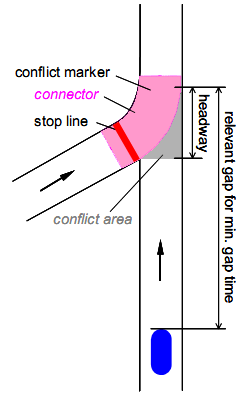
\includegraphics[scale=0.5]{priority_rules.png} 
\caption{From the Vissim manual: illustration of priority rule concepts}
\label{fig:priority_rules}
\end{figure}

In Vissim 5, which was used in this project, there is also the concept of conflict areas, which is recommended over priority rules (the latter remain in Vissim for compatibility) since they are easier to establish and will result in more intelligent driving behaviour. For instance vehicles will avoid entering a conflict area if they can see that it will not be possible to leave it with a certain minimum speed, which will prevent vehicles from clogging up intersections.

Conflict areas and priority rules both rely on threshold values (gap) which road users will use to assess wether it is possible to safely enter a conflict area. The gap is an estimate of the minimum time before the next vehicle from a conflicting link will enter the conflict area.

For the extensions made from Jyllingevej to Roskildevej relevant conflict areas was added for each of the four intersections. The default values in Vissim service pack 6 was used for all conflict areas.

During simulation it became apparent that the priority rules did not prevent collisions in the preexisting intersection so it was decided to replace them with conflict areas. The intersection which had collisions using only priority rules are:

\begin{itemize}
\item Herlev Syghus
\item Hjortespringvej
\item Herlev Hovedgade
\item Mileparken
\item Ejby Industrivej
\item Ejby Industrivej
\item Ejby Torvevej
\item Jyllingevej
\end{itemize}

The intersections with the most observed collisions were Herlev Hovedgade, Hjortespringvej and Herlev Sygehus. It appears that priority rules has difficulties in coping with trapped traffic whereas conflict areas avoid all collisions.
Thus the only priority rules which are carried over from the original model are those for bus stops. 

Conflict areas basically make vehicles in conflicting traffic flows aware of each other so that collisions can be avoided. It is also possible - but no mandatory - to assign a priority. Conflict areas for merging situations should preserve the order of the vehicles and thus have no priority. 

A number of additional situations arise for which the following rules were used:

\begin{enumerate}
\item Left-turning traffic must wait when traffic from the opposite direction - and in the same stage - is going through the intersection
\item When vehicles are trapped in the intersection, waiting for a left turn while the stage changes the vehicles from the next stage, which are in a conflicting motion, must wait for the left-turners to clear even though they have a green light. This is to avoid having traffic stuck in the intersection waiting for their next stage
\item Buses leaving bus stops are always prioritized
\end{enumerate}

\newpage
\section{Vehicle Actuated Programming in Vissim}
\label{vap}
VAP is an optional module for Vissim which enables direct programming of signal controllers. VAP is a simple, label-based (goto) language. The main feature is access to a library of functions, which manipulate the state of the signal controller. 

With VAP there is a graphical program, VISVAP, that allows the user to design a flowchart description of the controller logic, rather than writing it in VAP, as VISVAP can compile the flowchart into VAP. Figure \ref{fig:visvap_example} shows an example of a simple logic to control the lights at the ring 3 / Herlev Sygehus intersection.

\begin{figure}[ht]
\centering
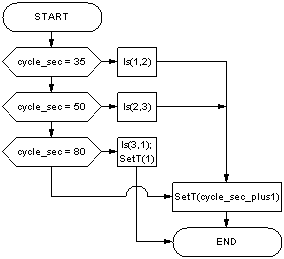
\includegraphics[scale=0.5]{visvap_example_herlev-sygehus.png} 
\caption{VISVAP flowchart description of simple fixed-time logic for Herlev Sygehus / ring 3}
\label{fig:visvap_example}
\end{figure}

The VAP program is called once for every simulation second. The starting label is START and the program proceeds as indicated by the arrows until the END label has been reached. Diamond boxes are logical tests where the right-going arrow indicates TRUE and down-going indicates FALSE. Square boxes contain expressions, in this case we use \verb|Is(<stage_from>,<stage_to>)| to switch between stages, when a certain portion of the current cycle time has passed. Below is the VAP code, which corresponds to the flowchart:

\begin{verbatim}
/* EXPRESSIONS */ 
            cycle_sec := T;
            cycle_sec_plus1 := cycle_sec + 1;

/* MAIN PROGRAM */ 

S00Z001:    IF cycle_sec = 35 THEN
S01Z001:      Is(1,2)
            ELSE
S00Z002:      IF cycle_sec = 50 THEN
S01Z002:        Is(2,3)
              ELSE
S00Z003:        IF cycle_sec = 80 THEN
S01Z003:          Is(3,1); SetT(1);
                  GOTO PROG_ENDE
                END
              END
            END;
S02Z004:    SetT(cycle_sec_plus1)
PROG_ENDE:    .
\end{verbatim}

VAP is unsuited for complex controller logic, such as ones involving predictions and optimization by iteration. This is due to the fact that VAP only has support for basic programming language constructs and the label-based nature of the language, which is detrimental to larger code bases see eg. the statement by Dijkstra \cite{nogoto}. As an example the above VAP code could be simplified into:

\begin{verbatim}
function UpdateController(cycle_second){
   switch(cycle_second){
   case 35: Interstage(1,2)
   case 50: Interstage(2,3)
   case 80: Interstage(3,1); Set_cycle_second(1); return
   case else:  /* do nothing */
   }
   Set_cycle_second(cycle_second + 1) /* update time */
}
\end{verbatim}

VAP is suitable, however, for implementation of DOGS due to its simple decision system as described in section \ref{dogs}. In this section I will describe how the DOGS logic was implementated in VAP.

\subsection{Interstage Definitions - PUA}
Before we move on to DOGS in VAP it is fundamental to explain the \verb|Interstage| (abbr. \verb|Is|) concept. Interstage definitions are mandatory in Vissim whenever a VAP program is to control a signal.

An interstage is basically the lighting scheme to be used during stage transition. Usually, when switching from stage A to B the lights of A switch to amber and then red while B switch from red to red and amber and then green.

The amber light of A is a warning that a transition is in progress, the intersection should be cleared and no more entries should be made. To ensure right-of-way consistency during the transition, B will stay red until the moment A switches from amber to red. For all intersections discussed in this project, the amber period is 4 seconds.

The red and amber period of B indicates that attentive entry into the intersection is permitted. The red and amber period is 2 seconds for all intersections.

Thus a total stage transition will last 6 seconds. In Figure \ref{fig:lost_time_example} is an example of the interstage lost times for various number of stages and cycle times. Some stages - eg. a through, left and rightgoing stage followed by a left-only stage - will be \textit{compatible} ie. there is no pause during the transition thus the table is pessimistic. However it clearly shows that there is a tradeoff between lost time and cycle time - especially in complex, multistaged intersections.

\begin{figure}[ht]
\centering
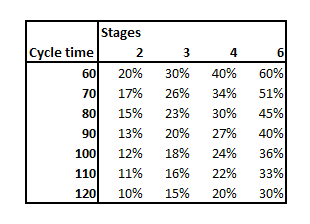
\includegraphics[scale=0.6]{interstage_lost_time.png} 
\caption{Interstage lost time in percent of cycle time for some combinations of cycle time and number of incompatible stages}
\label{fig:lost_time_example}
\end{figure}

In the above flowchart and code examples we start an interstage whenever we wish to move to the next stage.

The interstages are defined in Vissim by .PUA files. Below is an example of such a definition for Herlev Bygade. This intersection has two stages; stage A allowing traffic in either direction of the arterial and stage B for turn-ins from the minor road. 

\begin{verbatim}
$SIGNAL_GROUPS
A   1
B   2

$STAGES
Stage_1   A
red       B
Stage_2   B
red       A

$STARTING_STAGE
Stage_1

$INTERSTAGE1
Length [s]	 :   6
From Stage	 :   1
To Stage	   :   2
$    redend   grend
A    -127     0
B       4     127

$INTERSTAGE2
Length [s]	: 6
From Stage	: 2
To Stage	: 1
$    redend   grend
B    -127     0
A       4     127
$END
\end{verbatim}

In section \$STAGES it is defined that stage A should be green while B should is red and vice versa (they are not compatible). Here A and B refers to a space-separated list of signal groups from the \$SIGNAL\_GROUPS section.

For the interstage definitions, in INTERSTAGE1, we have redend for A to be -127, which means that A is green before the interstage, and grend (green end) is 0 meaning it should be red when the interstage has completed. For stage B, which is red before the interstage is run due to the \$STAGES definition, the redend (=green start) occurs 6 seconds into the interstage and grend set to 127 means that B should remain green after the interstage.

It is always up to the interstage designer to ensure that no right-of-way conflicts are present in the stage definitions. PTV supplies a support tool, which solves this issue, called CROSSIG. CROSSIG is capable of generating .PUA files; in this project CROSSIG was not available, however, and they were generated automatically from the signal plans, which are listed in appendix \ref{app:signalplans}.

\subsection{Interstage rules}
The signal plans, for which interstage definitions are to be built, are formatted so that each named signal group (head) has a row with $C$-cells, where $C$ is the cycle time. Each cell can be amber, green, yellow or red. Thus a complete signal timing plan is visually represented as one or more such rows in a stack.

In order to generate the interstage definitions (.PUA files in Vissim) it is necessary with a definition of an interstage itself. A stage is said to \textit{run} while the signal groups of the stage is settled in the green state. We define that when a stage is running an interstage cannot run and vice versa. Thus every cycle second must specify the current stage or interstage.

An interstage runs whenever one or more signal groups receive new colors until the changes of color have settled. This could for instance be the green end for group A, which is the start of an interstage cycle second the group begins to show yellow, until the perpendicular group, B, has settled its green light, which could include amber time. In the sample .PUA file above we see the implementation of this exact scenario: A ends its green time in interstage second 1 and B begins its amber-green time 4 seconds later, while group A is showing yellow. Group B shows amber for 2 seconds and thus the total length of the interstage is 6 seconds. 

It is important to note that, while stages must have a temporal extend to make sense, interstages may have zero length. Such interstages occur when light switch directly from red to green (respecting safety) and from green to red without the ordinary amber and yellow time respectively. Amber and yellow times are defined in the Vissim network file (.INP) and cannot be controller in the interstage definitions. Amber and yellow time is automatically appended by Vissim to the green- and red end times when the VAP controller runs an interstage.

A safety period, where all heads are red, is sometimes introduced in order to allow the intersection to be cleared. This can be modelled either as a stage with no green signal groups or included into the interstage definition by prolonging red end times and interstage length by the length of the safety period. The latter solution is preferred since it is directly supported in the PUA format and also avoids the introduction of an all-red stage and a number of extra interstages to and from the all-red stage.

\subsection{DOGS}
As VAP does not permit the writing of a program, which supervise all signal controllers at the same time, it was necessary to dedicate a signal controller as the master controller. To fully separate the master/slave concept it was chosen to install a virtual signal controller, whose only purpose is to run the DOGS program.

The master controller, which for the purpose of offset has a virtual location on Herlev Hovedgade, runs the DOGS program and determines the current level by inspecting the northern- and southern detectors according to the specification outlined in section \ref{dogs}. In addition this controller also runs the master clock and the current DOGS level and master cycle second is sent to all slave controllers every cycle second.

The slave signal controller - even the one on Herlev Hovedgade - must listen for communication from the master controller and set the green time of the various stages according to the current dogs level and cycle second as received from the master.

Both master and slave VAP controllers are generated automatically using a script, which takes parameters such as, for the master, the area-specific detectors and activation / level-up / level-down bounds and, for the slave, offset value(s), signal program etc.

\subsubsection{Master}
Relevant to master controllers we need to know the northern and southern detector names as these are used to determine if DOGS is enabled or turned off. Once DOGS is enabled another set of detectors (possibly overlapping) are measured upon to determine the appropriate level of DOGS. Note that, depending on threshold values, DOGS may be \textit{enabled} but not perform adjustments to the base-program - this is by design.

These threshold values are also parameters which is fed into the generator routine (see section \ref{dogs} for a description). 
Due to variations between the traffic, which TTS used to tune the threshold values, and the traffic which is observed in the simulation, it was decided to manually retune the vehicle count thresholds while keeping the thresholds for occupancy. 
Along with the detector data described in section \ref{detector_data} TTS supplied the selected DOGS levels in the same period. By a manual, iterative process the levels selected by DOGS in the simulator was fitted to the levels of the detector data set during the morning period. The main fixpoints used was the maximum and the average levels chosen.

DOGS accumulate detections over a cycle - which is of variable length - and compare to the threshold values. Occupancy is a the percentage of time of which the detector was enabled ie. a vehicle passed over or was in queue over the detector and thus the detection period can be chosen freely. The amount of vehicles which passed over (the 2nd component for threshold matching) is in total numbers and consequently when the cycle time increase so does the number of detected vehicles. TTS informs me that no adjustment - except for the standard exponential smoothening - is performed when comparing detector vehicle count values with the thresholds. I decided to correct this in the VAP code by assuming the counting thresholds matched a 80 seconds cycle and then scale the detected count to this level by using the actual cycle time (which is usually higher, when DOGS is enabled).

When DOGS is active the level is adjusted at most by one for each cycle. Thus when the level is high it will take longer to change between levels and the measuring periods are longer, resulting in more accurate measurements, but less responsiveness.

\subsubsection{Slave}
The purpose of slave controllers is to obey the cycle second and DOGS level instructions from the master controller.

The first step for a slave is to calculate the local cycle second, which due to controller offset will usually differ from the master cycle second. An exception is the slave controller, which controls the intersection in which the master controller is physically positioned - the distance between them is 0 and likewise the offset.

Consider stage A which is active while the master controller lowers the DOGS level by 1. In this case the end time is lowered if stage A receives priority from DOGS and it may happen that the end time for stage A is now lower then the current cycle second. Stage A will then have received more green time than it was supposed to and the slave will immediately make the transition from stage A to the next stage, B. In case B is not the stage which was supposed to be active (a rare case - stage B is short indeed) we allow stage A to carry over to the next cycle as we can only make stage transitions between subsequent stages - not in arbitrary order.

\subsection{Bus priority}
Three intersections in the Glostrup area - Fabriksparken, Gammel Landevej and Kindebjergvej - operate with bus priority on the arterial direction. 

If a bus arrives from north or south during the stage which belongs to the arterial green time of up to 10 seconds is distributed from the minor road stage to this stage. The effect is that buses might just make it across before the next stage is started rather than being cut off. In the next cycle the main stage is shortened by the same amount of time and the minor stage is lengthened accordingly.

This is implemented by associating detectors for north- and southgoing buses for each of these intersections. The autogenerated VAP code will then check for bus detections in each cycle second and perform bus prioritization if:

\begin{enumerate}
\item The main stage is the currently active stage
\item The signal controller is not currently performing a bus prioritization
\item The signal controller is not currently compensating the minor road stage due to prioritization in the previous cycle
\end{enumerate}

When bus prioritization is activated under these conditions the stage end times will be adjusted as mentioned and the next cycle (compensation) will perform likewise adjustments albeit inversed.

In case that a bus arrives and activates bus prioritization but make it across the intersection before the green time for the stage has been extended, bus prioritization is cancelled.
\newpage
\section{Traffic Analysis}
\label{data}
For the two areas of interest, Glostrup and Herlev, TTS supplied data from detectors for a period of a couple of weeks in november 2007. 

This period is generally accepted as the beginning of the winter season and as such the traffic is expected to be high.

The data from TTS is a supplement to the traffic counts, which were made available by DRD. Since the detector data is anonymous with respect to vehicles types, for links in the ends of the arterial (Herlev Sygehus from north and Roskildevej from east, west and south) the data from the corresponding detectors was used in the project to scale the input sizes of the traffic counts.

The format of the data from TTS is:

\begin{table}[ht]
\centering
\begin{tabular}{c|c|c|c|c}
\textbf{Date} & \textbf{Time} & \textbf{D1} & \textbf{...} & \textbf{DN} \\ \hline
13-11-2007 & 08:42:56 & 39 & ... & 35 \\
13-11-2007 & 08:44:26 & 38 & ...  & 28 \\
\end{tabular}
\caption{Format of TTS supplied detector data}
\label{tab:dataformat}
\end{table}

Thus each detector, named D\textit{N}, has a column where the numbers are the detected vehicles since last detection. The detections are made once for every cycle thus there will be some variations in the time between measurements due to the adjustments to cycle time, which are made by DOGS.

It was agreed with DRD that the temporal resolution for link inputs and route decisions was to be fixed at 15 minutes, which corresponds to the resolution of the traffic counts. Accumulation was performed on the DOGS data by indexing time within the data period into 15 minute bins and summing detections from the last 15 minutes.

Multiple data files - for different sets of detectors - were received for each area. Since the data period was not identical over the data files it was necessary to perform some cleanup in order to generate accumulated data in which all detectors were represented.

\begin{table}[!ht]
\centering
\begin{tabular}{c|c|c|c}
\textbf{Area} & \textbf{From} & \textbf{To} & \textbf{Detectors} \\ \hline
Herlev & 13-11-2007 20:45 & 28-11-2007 09:45 & D3-D8, D13-D15, D18 \\
Glostrup & 13-11-2007 08:45 & 26-11-2007 14:15 & D1-D14 \\
\end{tabular}
\caption{Periods of aggregated and cleaned data sets}
\label{tab:dataperiod}
\end{table}

The cleaned data was exported to a single table of more than 30.000 rows in the format:
\begin{table}[!ht]
\centering
\begin{tabular}{c|c|c|c|c|c}
\textbf{Date} & \textbf{Time} & \textbf{Area} & \textbf{Detector Name} & \textbf{From Direction} & \textbf{Vehicles} \\
\end{tabular}
\caption{Format of cleaned data set}
\label{tab:cleandataformat}
\end{table}

In the next section I will use the cleaned data to make some analyses and comparisons of the areas to discover facts on \textit{directional proportions} and \textit{distribution of traffic on a daily basis}.

Section \ref{traffic_count_analysis} brings additional conclusions from the traffic count data set to fill out some details, which cannot be extracted from the analysis of detector data alone.

\subsection{Detector data analysis}
\label{detector_data}
The first four graphs (Figures \ref{fig:proportions}) shows the overall fluctuation of traffic (mean-value) on workdays and in weekends split on mornings (7-9) and afternoons (15-17) for north- and southgoing traffic (N and S resp.).

\begin{figure}[htbp]
\centering
\subfloat[Herlev - morning]{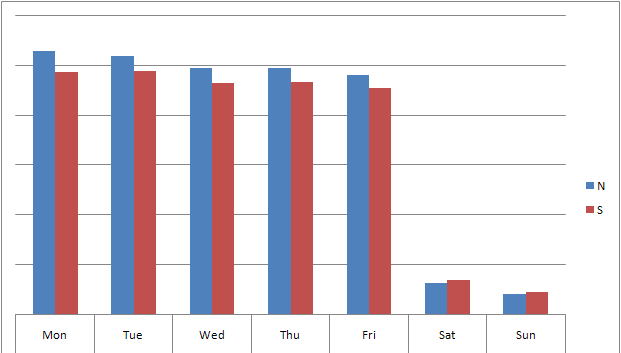
\includegraphics[width=\doubleimwidth]{herlev_direction_proportions_morning.png}}
\subfloat[Herlev - afternoon]{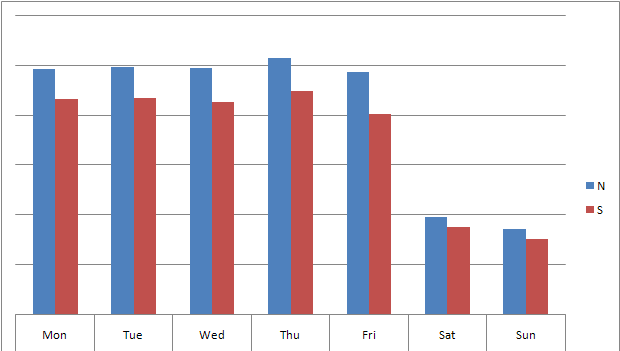
\includegraphics[width=\doubleimwidth]{herlev_direction_proportions_afternoon.png}} 

\subfloat[Glostrup - morning]{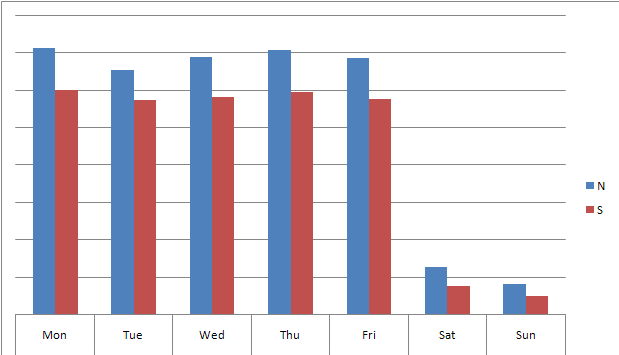
\includegraphics[width=\doubleimwidth]{glostrup_direction_proportions_morning.png}}
\subfloat[Glostrup - afternoon]{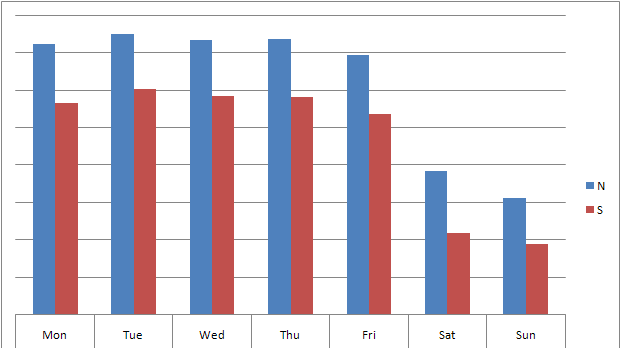
\includegraphics[width=\doubleimwidth]{glostrup_direction_proportions_afternoon.png}}

\caption{Proportions of north- and south-going traffic in the morning and afternoon in Herlev and Glostrup}
\label{fig:proportions}
\end{figure}

We can see that there is an overweight of northgoing traffic. This overweight is more profound in the Glostrup area and increases in the afternoon for both areas.

From these graphs we can also see that, in the weekend, most traffic happens in the afternoon.

The next graph, see Figure \ref{fig:commuter}, shows the usual commuter- and lunch traffic patterns. The data from all mondays to fridays in the dataset have almost identical temporal distributions and thus the graph shows summarized data from workdays.

\begin{figure}[htbp]
\centering
\subfloat[Workdays]{
   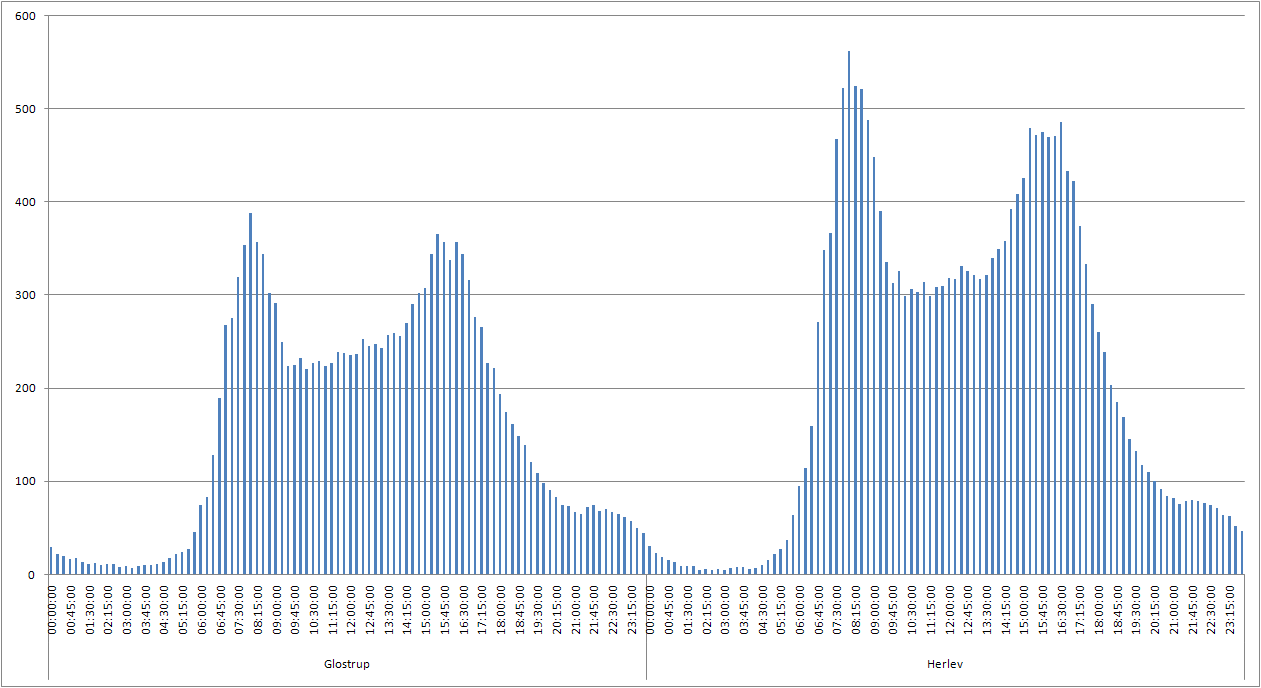
\includegraphics[width=\singleimwidth]{distribution_workday.png}
   \label{fig:commuter}
}

\subfloat[Weekends]{
   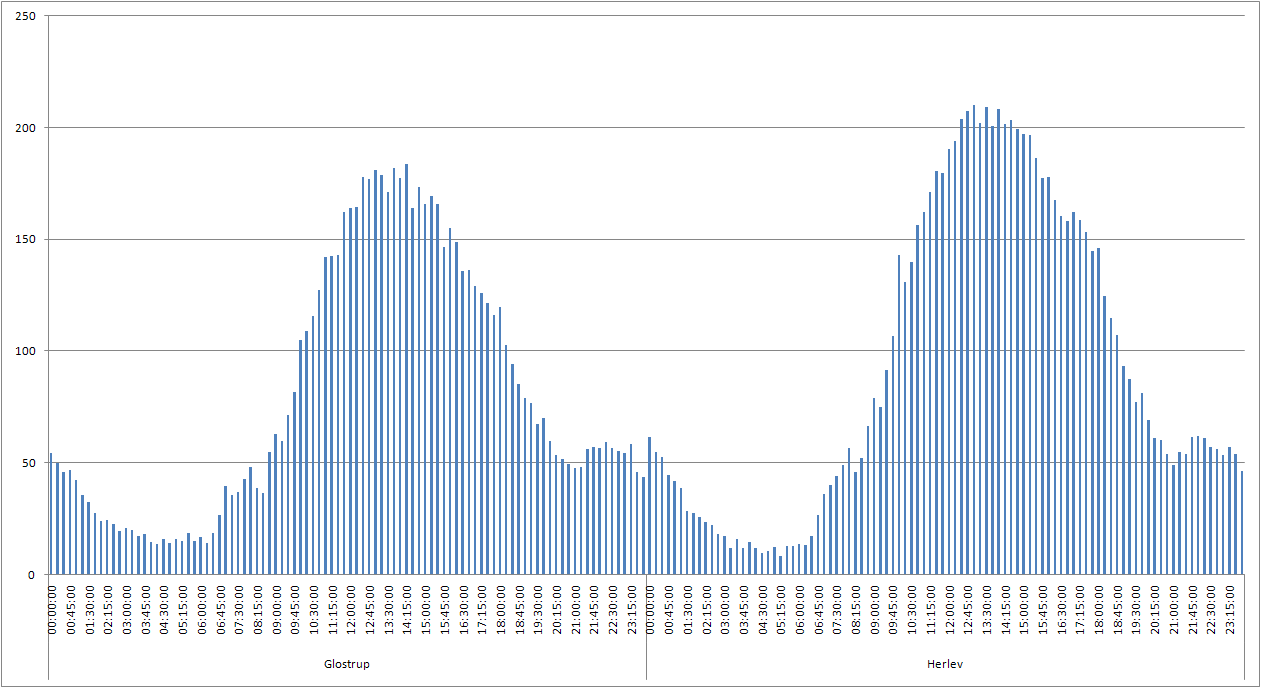
\includegraphics[width=\singleimwidth]{distribution_weekend.png} 
   \label{fig:weekends}
}
\caption{Distribution of traffic in Herlev and Glostrup}
\end{figure}

By comparing the workday distribution to the detected traffic in the weekend, see Figure \ref{fig:weekends} - and at the same time looking at the directional proportions - it is clear that ringroad 3 is heavily used by commuters in both Herlev and Glostrup. Traffic is almost identically distributed on saturdays and sundays and the graph shows summarized data for the weekend.


The next graph (Figure \ref{fig:detector_directions}) show how detections are aligned in the north and southgoing directions in both areas. (For both directions and areas these proportions do not vary in particular between workday and weekend).

\begin{figure}[htbp]
\centering
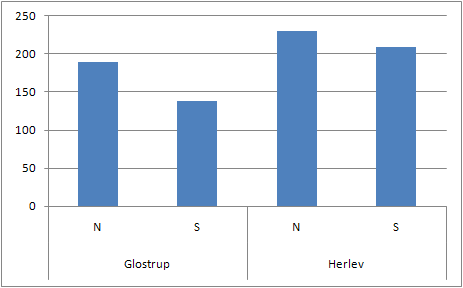
\includegraphics[width=0.6\textwidth]{detector_directions.png}
\caption{Relative detections for north- and southgoing links in Herlev and Glostrup}
\label{fig:detector_directions}
\end{figure}

One notable conclusion that can be drawn from these detector data is that there is a slight overweight of north-going traffic in both areas, in the most extreme case around 3:2, so the direction bias is not profound.

We can also conclude that ringroad 3 in Glostrup and Herlev face heavy commuter traffic by the classical increases in traffic from 7-9 and 15-17 but also slightly around 12 due to lunch traffic. The background traffic (ie. traffic not directly caused by commuters) through the workdays is heavy as well, starting around 6 and leveling off around 18. Morning and afternoon traffic appears to be quite similar.

\subsection{Traffic count analysis}
\label{traffic_count_analysis}

Traffic counts are widely used in traffic planning to setup simulations. They are performed manually by a suitable number of persons, so that each approach and turning motion of an intersection is counted simultaneously.

DRD provided traffic counts for every intersection except Ejby Torvevej (which is a blinded minor road and of little importance according to DRD) which has made it possible to model in detail the turning motions in the network.
The counting period was 7.00-9.00 in the mornings and 15.00-17.00 in the afternoons in 15-minutes intervals. The counts involved, for each approach, the turning movements of cars (including vans) and trucks. 

In Table \ref{tab:traffic_counts} we see a listing of the traffic counts and couting dates; most counts are from fall 2001 before the expansion of motorring 3 had begun. It is expected that the traffic has changed since then but the overall changes will probably fluctuate until motorring 3 is finished late 2008 (expected) due to differing conditions over time on motorring 3 (lane closures etc).

For some of the most important intersections (Mileparken, Jyllingevej, Roskildevej) we have newer traffic counts. For Herlev Hovedgade I received a detector count (MASTRA) from 2007 in addition to the traffic count in 2001, however the resolution was 1 hour and there was no distinction between cars and trucks and so it was disregarded.

\begin{table}[!ht]
\centering
\begin{tabular}{l|l|l}
\textbf{\#} & \textbf{Intersection} & \textbf{Date Counted}\\ \hline
1 & Herlev Sygehus & 30-10-2001\\
2 & Hjortespringvej & 09-10-2001\\
3 & Herlev Bygade & 04-10-2001\\
4 & Herlev Hovedgade & 02-10-2001\\
5 & Mileparken & 03-10-2005\\
6 & Ejby Industrivej & 27-02-2001\\
7 & Ejby Torvevej & -\\
8 & Jyllingevej & 23-10-2007\\
9 & Fabriksparken & 04-10-2001\\
10 & Gammel Landevej & 03-10-2001\\
11 & Kindebjergvej & 18-09-2001\\
12 & Roskildevej & 28-08-2003\\
\end{tabular}
\caption{Traffic count dates}
\label{tab:traffic_counts}
\end{table}

The main feat of traffic counts is that the ratio of cars to trucks is available. In Figure \ref{fig:cars2trucks} we see that - in total - there is about the same amount of traffic in each direction, however there are more trucks from south (ie. northgoing) supporting the results on direction bias from the DOGS detector data. Furthermore we are confirmed again on the clear arterial nature of the involved intersections due to the relative volumes of north-south going traffic to traffic from east-west.

The columns E and W indicate the total load of trucks and vehicles coming from east and west respectively, in which we see that the traffic from west, which is travelling towards the city of Copenhagen, is somewhat heavier than the traffic coming from east, travelling away from the city.

\begin{figure}[htbp]
\centering
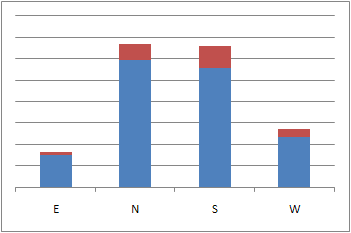
\includegraphics[scale=0.55]{cars_vs_truck_vs_direction.png}
\caption{Combined ratio of cars to trucks from each direction in the morning period. There are more trucks coming from south than from north.}
\label{fig:cars2trucks}
\end{figure}

In Figure \ref{fig:cars2trucks_time} we see how the proportion of cars and trucks evolve over time and note that the proportion remains the same in the sampling period.

\begin{figure}[htbp]
\centering
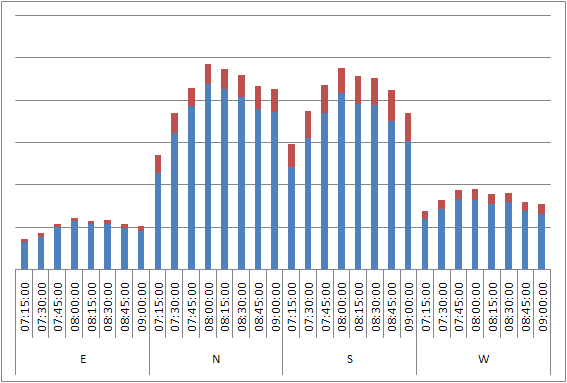
\includegraphics[scale=0.55]{cars_vs_trucks_vs_time_morning.png}
\caption{As Figure \ref{fig:cars2trucks} but over time. The proportion of cars to trucks does not vary much.}
\label{fig:cars2trucks_time}
\end{figure}

In the next figure (\ref{fig:cars2trucks_insect}) we see the proportions of cars to trucks for each intersection. The bars are the sum of cars and trucks in the morning period and also give an indication of the load each intersection faces. We can see that the most heavily loaded intersections are Herlev Hovedgade, Jyllingevej and Roskildevej (disregarding that two latter two were counted later than the other intersections) and that Herlev Hovedgade is the junction which sees the most trucks per car while Jyllingevej serve considerably less trucks. It is interesting to see that these heavily loaded intersections are the ones which were recounted after 2001, except for Mileparken.

\begin{figure}[htbp]
\centering
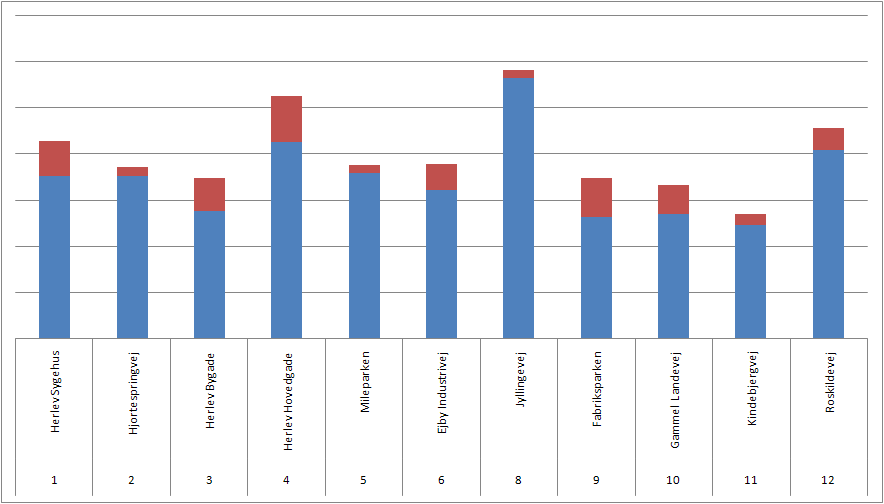
\includegraphics[scale=0.40]{cars_vs_trucks_all_intersections.png}
\caption{Cars to trucks proportions per intersection}
\label{fig:cars2trucks_insect}
\end{figure}

The final two figures (\ref{fig:insect_herlev}-\ref{fig:insect_glostrup}) show, for each DOGS controlled area, the demand faced from each direction split on trucks and cars. 

\begin{figure}[htbp]
\centering
\subfloat[Herlev]{
  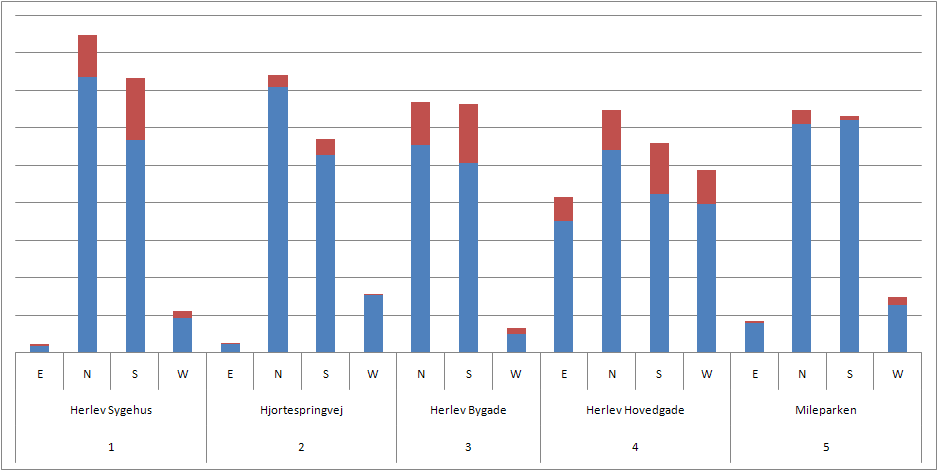
\includegraphics[scale=0.35]{demand_from_direction_per_intersection_herlev.png}
  \label{fig:insect_herlev}
} \\
    
\subfloat[Glostrup]{
  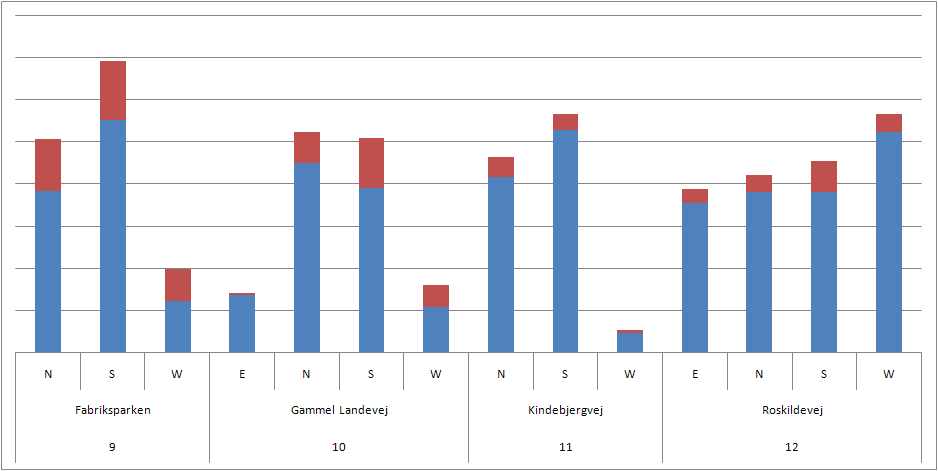
\includegraphics[scale=0.35]{demand_from_direction_per_intersection_glostrup.png}
  \label{fig:insect_glostrup}
}
\caption{Demand from direction per vehicle type in each area}
\end{figure}

In all cases the demand from cars by far outweighs truck demand; the intersections facing the most truck demand in Herlev are Herlev Hovedgade (from all directions), Herlev Bygade (from north and south) and also Herlev Sygehus from the arterial directions. 

In Glostrup we see that Fabriksparken has far more northgoing traffic and fair amounts of trucks and both arterial directions. Roskildevej has almost as much traffic from the sideroads as does Herlev Hovedgade, emphasizing the fact that ringroad 3 is not exclusively an artery in the north-south directions for several intersections.

\newpage
\section{Vissim Network Modelling}
\label{modelling}
The Vissim network used throughout the project is derived from a network originally started COWI and later reworked by DTU Transport students.

COWI's version included O3 from Jyllingevej to the intersection with highway 3 and even further north. In addition highway 3, which runs almost parallel with O3 in this area, was included as well as the minor roads in between.
The network was setup with dynamic assignment of traffic.

\subsection{Modifications \& Additions to Existing Model}

As such the network was missing four intersections of O3 from Jyllingevej to Roskildevej. To establish this section satellite photos from Google Earth was combined with intersection layouts, kindly provided by DRD.

The signal plans and naming conventions for the existing intersections in the COWI model for O3 intersections were adopted when entering the four missing intersections into the network. As for the intersection layout, DRD provided the missing signal plans for these intersections as well.

To prevent side-effects all links not connected to O3 from Herlev Sygehus to Jylligevej were removed as well as all parking lots (DTA zones).

\subsection{Link Inputs}

Due to the arterial nature of the Herlev area there is a natural distinction between major and minut link inputs. The major inputs are positioned in the ends and minor inputs are placed for each minor road.

In the southgoing direction vehicles entering the arterial from highway 3 and the northern extension of O3 are represented by a single input positioned before the intersection at Herlev Sygehus and would be detected by D3.

Northgoing traffic input is defined on the link leading to the Mileparken intersection and is detected by D14. 

The relative size of the major inputs are set according to the relative directional distribution seen in Figure \ref{fig:herlev_props} ie. 45\% northgoing and 55\% southgoing. XXX Insert more specific figure XXX

As the available dataset does not include detectors on the minor sideroads - from either side of the arterial - it is difficult to assess the relative size of the inputs from them. Thus for the remaining roads adjacent to the arterial are defined minor input links of identical size with the exception of the Herlev Sygehus link, which is set to be double the size to match the observations made above.
It is arguable that much traffic enters at the Herlev Hovedgade intersection, but the detected traffic does not indicate that this is significant.

The combined traffic input is set so that in total 20\% arise from the minor roads and the remainder enters from the ends of the arterial. 

XXX Try to find something to back this up eg. from Steen Lauritzens report XXX.

\subsection{Routes}
\label{routefractions}
In the network there exist a large number of routes which road users may take. The most obvious routes go all the way through the arterial but other likely routes go from a heavy-traffic minor-road such as Herlev Hovedgade and exit at either at one of the ends of the arterial or at another heavy-traffic minor-road such as Jyllingevej.

At every intersection it is possible to follow each adjacent link (ie. turn left, right or go straight through) and thus the total number of routes from an input link to an exit link in the network is tremendous.

DRD provided traffic counts for every intersection except Ejby Torvevej (which is a blinded minor road and of little importance according to DRD) which has made it possible to model in detail the turning motions in the network.
The counting period was 7.00-9.00 in the mornings and 15.00-17.00 in the afternoons in 15-minutes intervals. The counts involved, for each approach, the turning movements of cars (including vans) and trucks. 

To apply this dataset in Vissim it is possible to use \textit{turning decisions} but the Vissim manual is clear that static routes should be used (rather than turning decisions) when modelling turning distributions. The main reason is that congestion may cause a decision to turn to be overruled whereas a vehicle on a fixed route will wait for the congestion to clear. 

The simplest approach was to introduce a routing decision for each approach, which had traffic count data, and then add routes - respecting the counting data - which represented the turning motion. Such a route is \textit{internal} as it does not necessarily lead from an input to an exit link. Consequently this approach yields a network with the possibility of endless circulation, however since we only regard an arterial in this project - and the fact that there are no U-turns in the network - no vehicles will be able to circulate and will always find an exit link.

The routing decision must be placed at a \textit{decision point}, however this does not exist in Vissim. Rather the decision point is scattered over 2 or more connectors attached to each link facing an intersection. In order to overcome this these connectors were grouped by a naming convention which identifies which decision point they belong to and which turning motion they will cause a vehicle to take. 
The names are the concatenation of the direction from which traffic arrives (ie. north, south, east or west), the number of the intersection the decision belongs to (intersections are numbered increasingly from north to south) and finally the turning motion (ie. left, through or right), whichever is applicable. 

As an example the decision point at Herlev Sygehus (intersection 1), which faces traffic from north consist of three connectors, are called \verb|N1L|, \verb|N1T| and \verb|N1R|.

To find the insertion point for the routing a backtracking search is made from each turning motion until a common link is found. This link is thus the decision point and we can automatically generate our internal routes by using the discovery routine of section \ref{routingdecisions} to find a valid route.

In Figure \ref{fig:flow_dist_principle} is an example of decision points (y) and the proportions of traffic for each turning motion.
\begin{figure}[!ht]
\begin{center}
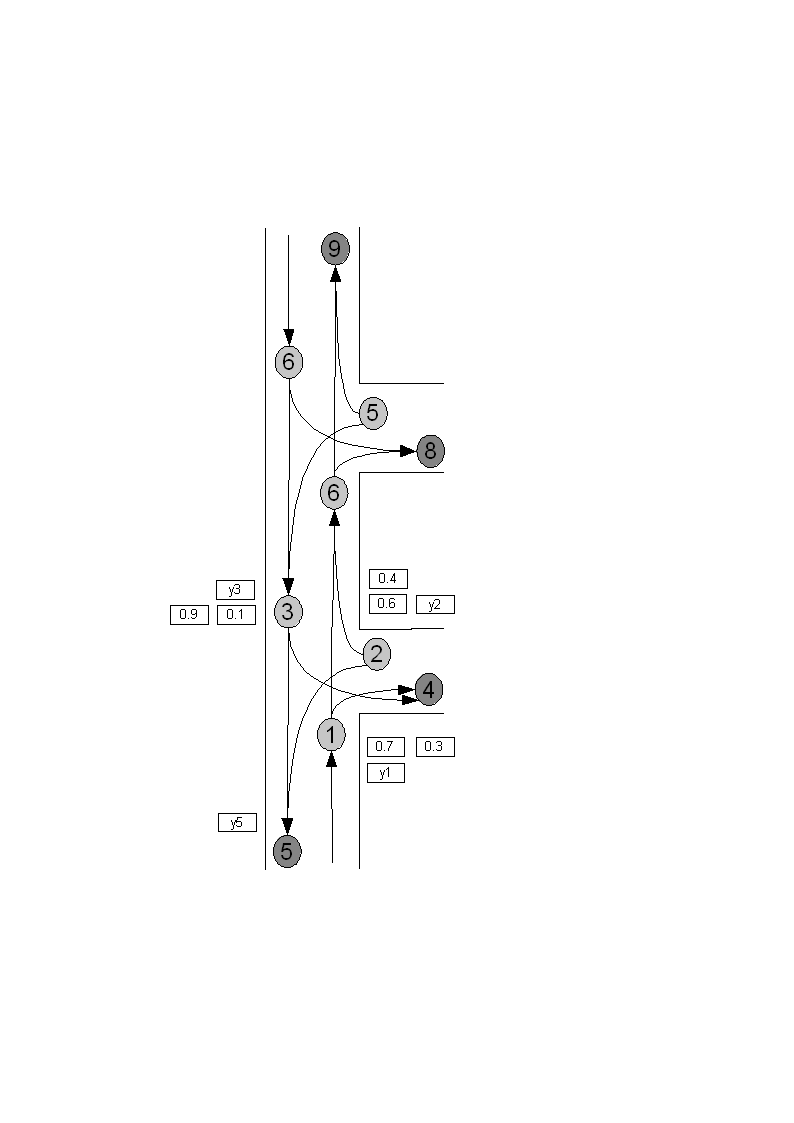
\includegraphics[scale=0.6]{trafficcount_to_routes_sketch.png} 
\end{center}
\caption{Flow distribution principle}
\label{fig:flow_dist_principle}
\end{figure}

\subsection{Signal Plans}
Signal plans define the stage sequence, green duration and how changes between adjacent stages should happen with respect to colors in the from and to stages. For cycle-based signal plans the cycle time must be equal to the sum of green and interstage time from the beginning of the first stage until it begins again.

A single stage defines the signal head colors of one or more signal group, which, in turn, is a group of signal heads operating synchronously.

The simplest signal controller consist of two stages. In  Figure \ref{fig:simple_intersection} the arrows indicate the directions being served green.

\begin{figure}[!ht]
\begin{center}
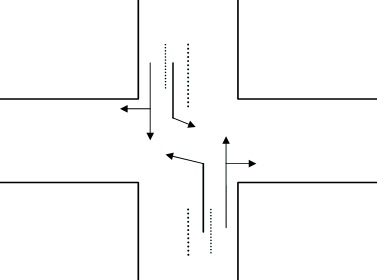
\includegraphics[scale=0.5]{simple_intersection.png} 
\end{center}
\caption{A simple intersection}
\label{fig:simple_intersection}
\end{figure}

DOGS rely on existing signal and modify the duration of the stage or stages, which serve green in the direction of the arterial. Thus DOGS assume that the stage sequence and interstages are \textit{optimized} so that the time lost in stage changes is minimized and \textit{safe} so that vehicles in eg. left-turning movements have time to leave the intersection before the conflicting direction receives green.

For this project DRD has supplied a number of signal plans for each intersection, developed by TTS. Throughout the plans signal groups in one direction (usually the major one) are named A and B in the perpendicular direction. Names such as At, AV, AtV indicates signal group for the throughgoing, leftgoing (V = venstre (danish) = left) and a combination for the final name variant. Lower case a's and b's indicate a signal group for pedestrians in the major and minor direction resp.

For some intersections a number of alternative plans were supplied. Considering the scope of this project only a single plan was chosen for each intersection and time of day. Generally plans involving pedestrian or bicyclist actuated stages were avoided so as to maximize the potential for traffic signal optimization. It was confirmed by TTS that these types of stages, which are taken in a stochastic manner ie. when a button is pressed, can be devastating to the coordination of traffic signals.

As a final simplifying step it was chosen not to provide signal heads for pedestrians and bicyclists as these types of road users are not being simulated. Pedestrian stages will mostly follow the parallel stages anyway and if this is not the case the stage, which is being denied in favor of the pedestrian stage, will simply receive red for the duration.

The final plans, which are used in the simulation, can be seen in appendix \ref{app:signalplans}.

The actual implementation was done in VAP by running the interstages at the cycle second according to the signal plan, for more details refer to section \ref{vap}.

\newpage
\section{Optimization System}
\label{optimization}
This section will discuss the alternative proposal for arterial optimization, which was developed in response to DOGS.

\subsection{Coordination}
\label{coordination}
Coordination along an arterial is fundamental in signal optimization. The ideal situation for road users is the \textit{green wave}, where upon arrival to the next intersection there will always be a green light.

Contemporary car engines consume less fuel in general when they are allowed to run at a constant RPM level so the travel experience as well as emmission levels are improved under coordination.

There are also security aspects which indicate that coordination and green waves are desirable since the human eye has difficulty in observing acceleration and deceleration.

In one-way coordination a signal controller emits a platoon of vehicles over a period of time, say from $t_1$ to $t_2$, where $T_g = t_2 - t_1$ is indicative of the number of vehicles that need to pass. To avoid stopping these vehicles at the next signal the same amount of green time, $T_g$ must be given to the approaching platoon only \textit{offset} in time by $o$ time units to represent the travel time of the platoon from one signal to the next. 

In fact, due to \textit{platoon dispersion} SEE XXX XXX, which depend mainly on the intersignal distance and speeds, more than $T_g$ green time must be allotted to the stage of the downstream signal. It is also due to platoon dispersion that coordination is only relevant for signals which are relatively close. Practical experience from DRD indicate that the distance should not exceed 800-900 m. 

In perfect two-way coordination between two intersections the leading vehicles in platoons of traffic in either direction must experience that the next signal switch to green before they reach the area in which they decide to brake for red.

In a common cycle-time based system \cite{coord} gives us:

$$o = n \cdot \frac{C}{2}$$

Where $o$ is the travel time between the intersections, which is assumed to be the same in both directions, $C$ is the cycle time and $n$ is an integer.

The travel time is calculated as $o = L / v$ where $L$ is the distance and $v$ is the speed by which road users travel between the intersections. By insertion we get:

$$C = 2 \cdot \frac{L}{n \cdot v}$$

This equation is quite constrained, however. For cycle time we require that is lies within a span of about 60 til 120 seconds based on recommendations from DRD. If the cycle time is less stage lengths become too short to reach past the queue startup delays (about 4 vehicles), if more the minor roads experience long delays and pedestrians and bicyclists may start to cross the road before the signal is green.

In addition green waves usually span over more than two intersections with may have different distances and average speeds between them, all this making it hard or impossible to find an integer $n$. Thus green waves are most obvious in one, main direction. It is possible to affect the average speeds between intersections by changing the allowed speed-signs. If this is not sufficient one might accept that the green wave is not perfect by, for instance, prioritizing one direction over the other.

Priority can be given entirely to one direction or distributed by some weight, for instance based on the ratio of traffic in each direction. An obvious choice for the first option would be for an arterial with traffic between some suburbs and a major city. In the morning full priority should be given in the direction towards the city when people go to work and opposite in the afternoon. A third alternative is to a perfect progression band in one direction for a some ratio of time, corresponding to the ratios of traffic in either direction.
For ring road 3, which was simulated in this project, there is no clear distinction between the direction of morning and afternoon traffic (see Section \ref{data}) and a solution which weights the green wave quality according to direction ratio. 

The distance between one signal head (intersection) and the next can be extracted from the Vissim network file in both directions and is static. The signal heads for both directions of the arterial are marked using a naming convention similar to the one mentioned in Section \ref{routefractions} only less information is required since the relation of the head to its signal controller can be deduced directly from the network file. Further details on this process can be read in Section \ref{signal_details}.

For travel times (which is a key component in finding a proper offset) it is possible to rely on the speed limitations / free flow speeds for offset calculation, however under congestion speeds will decrease causing the travel times to increase. A better solution is to continously inspect the smoothened travel times which are inserted for each stretch. 

\subsection*{Why are we using common cycle schemes?}
In this section I highlight the restrictions imposed when introducing two-way coordination between common cycle time signal controllers. Are there no alternatives, which are less strict and why aren't they used in denmark?

With a common cycle time comes fixed signal plans that give us full insight into the operation of the each signal controller. We can see exactly which signal groups ie. heads are green, red, yellow and amber at any give second. Furthermore, as presented above, there exist expressions for the offset and cycle time which causes coordination. 

Although traffic actuated green time extension schemes exist to make fine adjustsmens, such as the ones used for bus priority, it is always necessary to take the seconds from some other stage due to the common cycle time requirement. Likewise with stage skipping, you must always "spend" $C$ cycle seconds and may never spend more.

These restrictions makes it difficult for a computer system to obtain optimum performance for the signal controllers and the observed / predicted traffic.

Stage based signals is an alternative to fixed signal plans where stages are queued for future execution along with a green time. There is no fixed order of the stages and no fixed green time. This gives great flexibility for the computer system, however the problem is the plans cannot be written down in advance in terms of $C$ for human inspection and control. Instead they must be defined dynamically on the basis of a set of signal rules, which are implemented and respected by the computer system while adapting to the measured traffic conditions. 

Here are some rules such a system should implement:

\begin{description}
\item[Coordination]
Whenever the arterial stage for a signal is active from $t_1$ to $t_2$ the arterial stage of the downstream signal should be active from $t_1 + o$ to $t_2 + o$ where $o$ is the travel time from signal to signal 2.
\item[Priority for the arterial]
The green times for all stages in the direction of the arterial must match the load on the arterial, respecting other rules.
\item[Fairness to minor roads]
The queues for minor roads cannot exceeed a predefined length nor must a vehicle wait more than a certain amount of time at the intersection to pass.
\end{description}

These rules - given proper parameters - are precise enough to be implemented in a computer program. The setting of parameters (for instance maximum queue length for minor roads) is a difficult subject, which could generate many training hours for end-users. This was my impression about the Utopia/Spot system the municipality of Copenhagen (Vej \& Park) had implemented for Centrum Forbindelsen - they had no idea on how to make adjustsments, when the system acted up. 
However, many parameters can - and should - be set automatically by repeated simulation with trial-and-error or they are either easy enough to understand that rules of thumb and area specific insight is enough to make proper choices.

I believe stage based signals and more centralized computer control of arterials could be accepted and achieved if systems were more available and open as proposed above. The introduction of stage based signals would be a major break with tradition in denmark - and probably also in many other countries. 

Breaking tradition is always hard; this combined with the volume of such a system has compelled me to remain in the common cycle time world in this project. But as will be seen in the following sections, there are many ways to improve arterial signal performance in spite of the the restrictions of $C$.

\subsection{Manipulating speed}
The first option, which is implemented in the search procedure (see section \ref{siman}), is to improve coordination by affecting the speeds of road users. This is done by adjusting speed signs since most motorists will obey these. The travel time between intersections, which largely determines the offset, could then be increased or decreased by changing the speed signs. 

In Figure \ref{fig:change_speed} we can see how this works. In the \textit{before} situation, platoons from intersection $i+1$ arrive too late and some experience red light. In the \textit{after} situation, the platoon is allowed to go faster and arrive entirely during the green time of intersection $i$.

\begin{figure}[ht]
\begin{center}
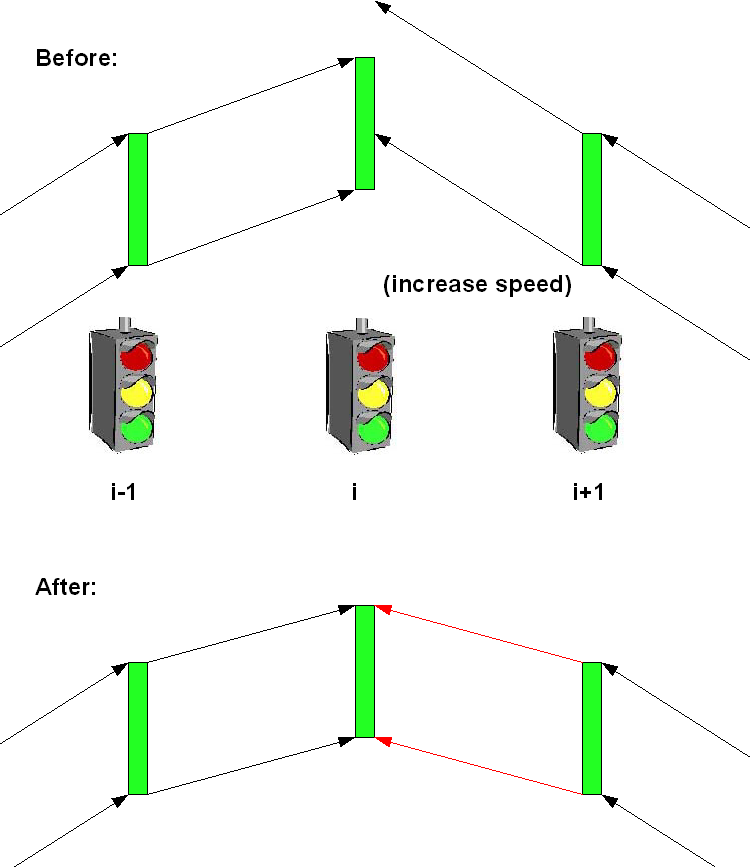
\includegraphics[scale=0.2]{change_speed.png} 
\end{center}
\caption{Changing speeds to obtain better coordination}
\label{fig:change_speed}
\end{figure}

Some considerations should be made in this respect. For instance we must ensure that the speeds do not divert too much from the norm of the relevant type of road. In addition the number of speed changes, which a motorist travelling throughout the arterial experience, must be minimized. And if speed changes do occur, it is a good idea to keep them small so that the speeds don't go from 50 to 70 from one stretch of road to the next.

From a security perspective it might seem risky to not persist a common speed level through the artery. But considering that a change of speed might improve the quality of the coordination, this problem is negated. This also applies to the additional acceleration and deceleration since, if a green wave does not exist the vehicles must be stopped altogether at the red light causing even more acceleration.

The current infrastructure on O3 does not offer this fine-grained level of adjustment but electronic speed signs are common practice nowadays and is, for instance, used on the almost-parallel motorring 3 to smoothen out queues.

\subsection{Adjusting offsets}
The individual signal offset is the traditional parameter for adjustment. The formulas presented earlier (section \ref{coordination}) can be used to establish one-way coordination, under the restrictions described, but two-way coordination is not solved so easily.

Basically the purpose of offsets is to properly align adjacent intersections in time such that a platoon emitted during the green time of intersection 1 is met by a green light at the adjacent intersection 2. The best estimate of the propagation time of the platoon is the travel time $tt_{1,2} = d / v$ where $v$ is the average speed and $d$ is the distance between the intersections and the green time displacement, $\Delta o_{i,j}$, should match $tt$ for all adjacent intersections $i$ and $j$.

\begin{figure}[ht]
\begin{center}
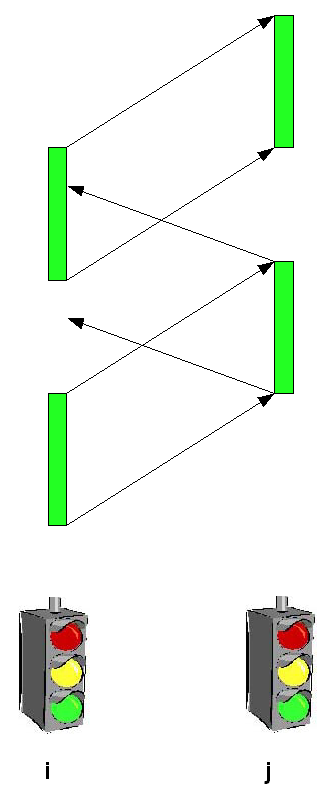
\includegraphics[scale=0.2]{change_offset.png} 
\end{center}
\caption{Changing speeds to obtain better coordination}
\label{fig:change_offset}
\end{figure}

We can change both the travel time, by changing speed signs, and also the green time displacement by adjusting offsets. The consequences of changing an offsets can be difficult to foresee, consider the example in Figure \ref{fig:changing_offset}. From intersection $j$ to $i$ the platoon will arrive too early. We can increase the offset (delay the green start) of $j$ but then we just reverse the situation. During all this, we must expect that there are also signal controllers $i-1$ and $j+1$ to the left and right resp. of $i$ and $j$, which must be in coordination with $i$ and $j$.

Metaheuristic search procedures are designed to cope with situations such as these where the immediate effects of a change cannot be foretold or enumerated.

\subsection{Metaheuristic Search}
DRD has traditionally used TRANSYT to obtain coordination. TRANSYT employs a genetic algorithm to finds its solutions but often it is necessary to manually adjust the offsets in order to obtain a good two-way coordination or to give preference to some direction. 

This manual process involves creating good two-way green waves by compromise, which could be either some sacrifice in the quality of the green waves. 

In this project the green wave concept has been formalized so that it is possible to evaluate a proposal for offsets. This opens up for the application of a metaheuristic search procedure.

In this first cycle-based approach the variable to be optimized is, of course, the offset for each signal controller. The signal controllers themselves operate under cyclic plans which are shifted in time according to the chosen offset. In addition the allowed speeds from a signal to the next may be changed to obtain better results.

\label{eval_coord}
For evaluation of a \textit{coordination} between $sc_1$ and $sc_2$ (directed) in the context of a time horizon $H = h_{min} .. h_{max}$ we examine each green band, which is emitted from $sc_1$. Given the distance and chosen speed from $sc_1$ to $sc_2$ we can count how many seconds worth of green band, which is not being let through by $sc_2$. The band from $sc_1$ may be cut in three ways, if $sc_2$ does not provide a green light, when the band reaches it 1) completely ie. there is a red light for the duration of the band 2) the front is cut off 3) the tail is cut off.

Obviously the first option is worst as all vehicles must halt. Second is the cutting of the leading vehicles, since they must brake or come to a halt, effectively halting the entire platoon. Least intrusive is the cutting of the tail, since then, at least, parts of the platoon actually experienced a green wave when travelling between $sc_1$ and $sc_2$.

\subsection{Simulated Annealing}
\label{siman}
In this section I describe the metaheuristic search routing, which was chosen: Simulated Annealing (SA). 
SA is a \textit{hill-climber} with the ability to escape from local optima ie. jump to another hill-top.

What this means is that SA performs a randomized, converging search in the entire search space (for offsets that is each combination of $N \bmod C$ over the intersections) looking for the possible best set of offsets without getting stuck with the \textit{first-and-best} solution it encounters.

The initial solution is chosen so that all offsets are zero. SA then works its way toward a better solution by examining neighbor solutions to the current one. A neighbor solution is found by incrementing or decrementing a single offset in the current solution or changing the allowed speed between the intersections by 5$km/h$.

The solutions to offsets are evaluated and compared in the context of the network and, if a neighbor is found to be better than the best solution found so far, it is adopted as the new \textit{encumbent}. If the neighbor was not better it should be thrown away, but here SA avoids being caught in a local optima by \textit{with some probability} keeping the neighbor solution regardless and work on from there. This probability will decrease as the search progress and so it is subject to tuning.

Generally metaheuristics give no guarantee that an optimum solution will be found, but with proper tuning and fast data structures, so that at least a couple of hundred solutions can be tested per second, it will generally yield good solutions. The strengths of metaheuristics are that they can easily support any kind of constraint, take advantage of the structure of the problem and run in O([insert seconds here]) ie. the running time is bounded by the time available.

In this project I have developed data structures, which are fast enough to generate the necessary iterations per second and can be used in various metaheuristic search schemes, not just simulated annealing.

The keys to speed in metaheuristic search are \textit{delta-evaluation} and to avoid \textit{object instantiation}.

\subsubsection{Delta-evaluation}
To evaluate a solution for offsets for sequentially adjacent signal controllers $sc_1$ to $sc_n$ we evaluate, in accordance to description in Section \ref{eval_coord}, each coordination $(sc_1,sc_2)$, $(sc_2,sc_1)$\footnote{Coordinations between adjacent signal controllers need not be symmetrical. For instance there might be a longer way in one direction that the other or, more likely, different \textit{speeds} might be allowed} and so forth. This gives us a value for each coordination and we then perform some kind of aggregation in order to obtain a single figure, the solution value.

Every time a neighbor solution is generated we normally immediately want to evaluate it as well. This can be done by going through the routine described above, but we can also use delta-evaluation to speed up the evaluation, if we have information on the structure of the problem.

A change in the offset of signal controller $sc_i$ will affect the coordinations between $sc_{i-1}$ and $sc_{i}$ and also between $sc_{i}$ and $sc_{i+1}$. Since we didn't change the offset $sc_{i-1}$ or $sc_{i+1}$ or any other offset, all coordinations but those mentioned will remain just as good - or bad - as before the offset change for $sc_i$. This is illustrated in Figure \ref{fig:delta_eval}.

\begin{figure}[!ht]
\begin{center}
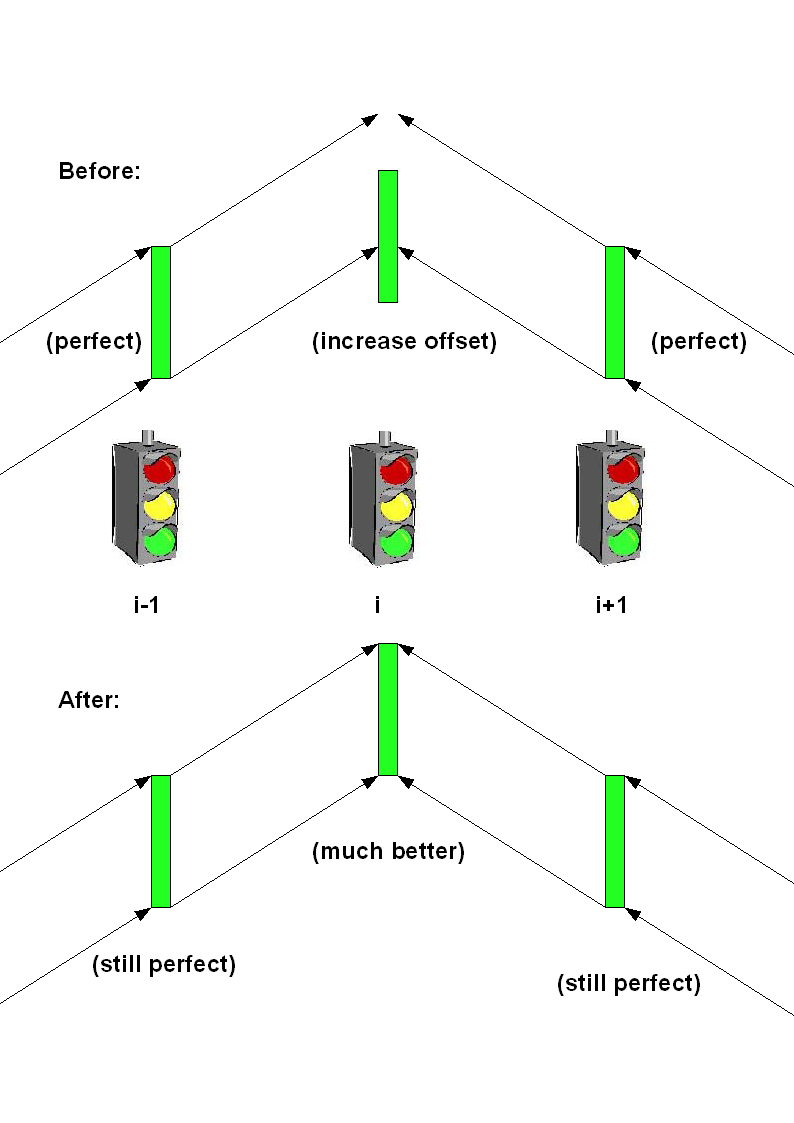
\includegraphics[scale=0.3]{delta_eval.png} 
\end{center}
\caption{Local nature of coordinations. This illustrates the quality of coordinations between three signal controllers before and after changing the offset of the middle controller. Notice that the coordinations between the outer controllers and $sc_{i-2}$ and $sc_{i+2}$ remain the same.}
\label{fig:delta_eval}
\end{figure}

So, rather than evaluating every coordination again we may safely assume that only coordinations $(sc_{i-1},sc_{i})$, $(sc_{i-1},sc_{i})$ and $(sc_{i},sc_{i+1})$, $(sc_{i+1},sc_{i})$ need to be reevaluated. 

We now need only to evaluate at most four coordinations\footnote{Changing offsets for controllers in the ends of the arterial will only change the value of two coordinations.} to obtain the neighbor solution value. In total there are $2\cdot (n-1)$ coordinations to evaluate since each signal controller has an outgoing coordination in each direction except at the ends, which have only one. Thus we exchange a linearly growing reevaluation time (in the number of signal controllers) for a constant one and rough tests have shown that, even for small networks, the savings are in excess of a factor two, in spite of the extra overhead due to bookkeeping.

\subsubsection{Neighbor solutions}
In previous studies of metaheuristics, where the object oriented programming model was completely adopted, it was found that the overhead of object instantiation, whenever a neighbor solution was generated, would result in tremendous time consumption. 

Instead I have minimized the need for copying information from a solution to its neighbor by introducing the dual methods \verb|change| and \verb|undo_changes|. The purpose of these methods is to allow a solution to temporarily take the form of its neighbor and switch back to its former self, if requested. 
When the metaheuristic runs it will constantly ask for neighbor solutions but throw away most of them. This approach avoids much copying of solution attributes and at the same time the details of the switching of identify are relayed to the solution object.

\subsubsection{Bookkeeping outline}
The \verb|change| and \verb|undo_changes| methods are closely integrated with delta-evaluation. The initial solution obviously cannot be delta-evaluated so, during full evaluation, the \textit{contribution} from each coordination is noted. 

When \verb|change| is called a signal controller whose offset to change is chosen as well as a new offset value. Next we find the affected coordinations and update the value of the solution by swapping the old contributions with the new ones, when evaluated under the changed offset.

We must be ready to undo the changes we just made, so we track all these changes: which offset we changed and by how much as well as the previous contributions from the affected coordinations.

The extra time spent on bookkeeping is bounded by the number of affected coordinations, as explained previously and does increase the complexity of the codes by a great amount.



\newpage
\section{Test Scenarios}
The purpose of this section is to highlight the findings in the various simulation runs which were performed.

The primary purpose of the simulation was to test the DOGS system against a theoretically better founded system for dynamic signal control. In addition tests were performed to discover the effect of bus priority and to determine whether DOGS with its varying cycle time can outperform a fixed cycle time but properly coordinated offsets.

All simulations were fitted to the traffic observed in the morning period fra 7-9 am.
To account for fluctuations each test was run 5 times with different seeds.

The results of the tests are measured by extraction of average queues and delays for each intersection. This is done by inserting a node with node evaluation enabled for each of the twelve intersections.

\subsection{The Effect of DOGS}
This test covers four scenarios:

\begin{enumerate}
\item DOGS and bus priority
\item DOGS without bus priority
\item Default program with bus priority
\item Default program with no priority for buses
\end{enumerate}

In scenario 1 and 2 DOGS is enabled and the capacity in the main direction is adjusted according to detector values. In scenarios 3 and 4 DOGS is disabled effectively ignoring all detections (except for buses in scenario 3) and thus the signals will remain in the base program.

As DOGS will naturally cause decreased performance for the minor roads it was decided to split the dataset so that \textit{arterial} and \textit{crossing} traffic can be distinguished. For delays arterial traffic is defined as traffic which enters an intersection from north or south and makes a throughgoing motion rather than turning off the arterial. All other traffic is marked as crossing.

\subsection*{Bus Priority}


\subsection{Coordination with Direction Priority Offsets}


\newpage
\label{sec:conclusion}

The emphasis of this survey has been on adaptive systems, which can
accommodate for the fluctuations in traffic.  The flexibility of the
model (or lack of it) underlying the optimization is a determining factor
regarding the level of adaptiveness that is achievable. The offline
optimization systems (section \ref{sec:offline}) all operate with the
common cycle time concept, which allows coordination to be set up by
offsetting downstream intersections. The common cycle time is
prohibitive when adaptive systems try to react to (predicted) arrival
of single vehicles or platoons of vehicles, even.

There are several models for traffic networks, which are not based
on the periodic behaviour of offline systems to perform
coordination. Instead they assign green time to phases in some order,
which is optimal given the detected and predicted traffic.  In section
\ref{sec:adaptive_cooperation} three systems were discussed in
detail. They were selected to give examples of adaptive control at
different levels (network, arterial and intersection). Two of them
(network and intersection control) use the direct assignment / phase
assignment methodology and the last (DOGS for arterial control)
operates with a classical model, but is designed so that the mentioned
problems are negligible.

DOGS is an example of a simple, but efficient, solution to dynamic
capacity adjustment for an arterial. It has been implemented for
multiple highway arterials and has thus proven that it can supply
capacity increases when needed as well as adjust priority to minor
roads once the traffic flow on the arterial diminishes.  DOGS has little
mathematical background, however, and has not been simulated prior to
implementation.  In a future project it would be interesting to
introduce a mathematical foundation for DOGS, preferably on the basis
on some established arterial progression scheme such as
REALBAND. Before and after scenarios could be simulated to determine,
what improvements are possible by going from a system adjusted by
ad-hoc methods to a truly optimized system.


\cite{*}

\newpage

\bibliographystyle{plain}
\bibliography{bibfile}

\newpage
\appendix

\section{Signal Plans}
\label{app:signalplans}
In this section you see the chosen and simplified signal plans for DOGS optimization.

\begin{figure}[!ht]
\begin{center}
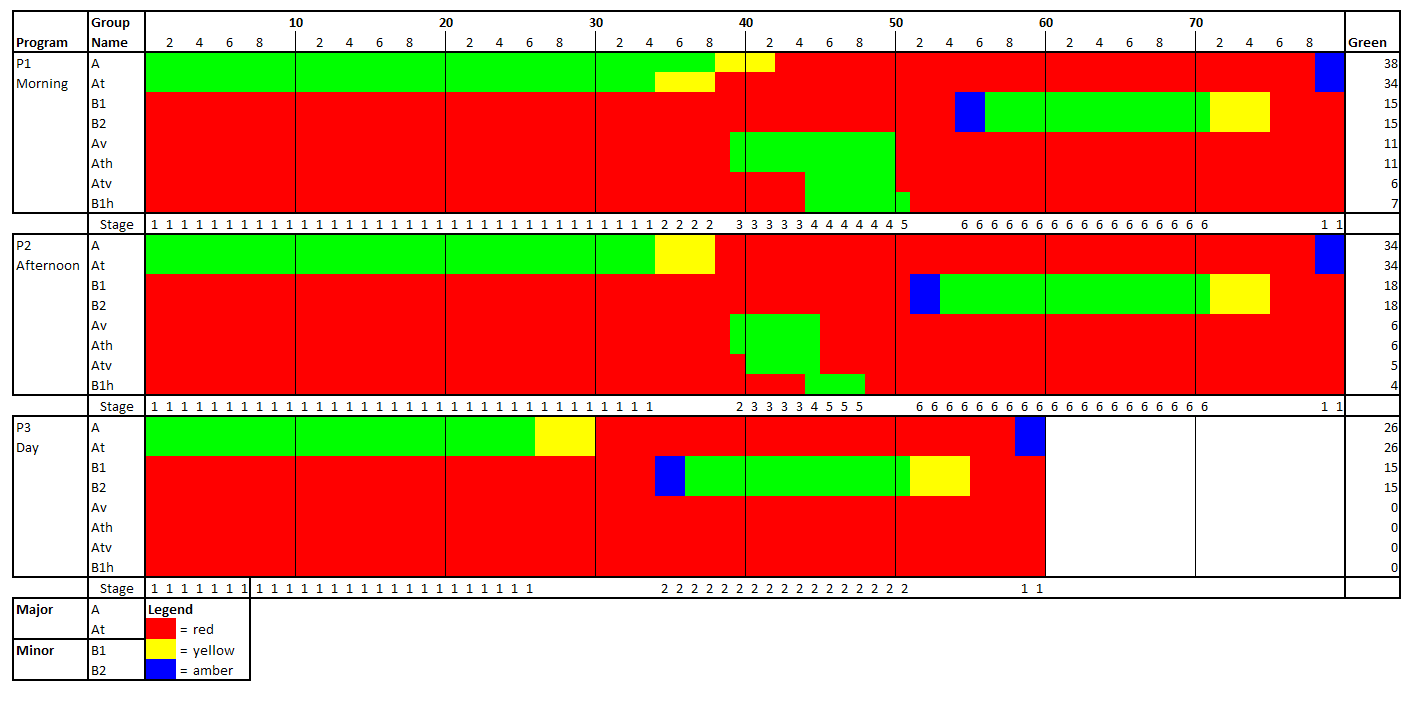
\includegraphics[scale=0.5]{sgp_mileparken.png} 
\end{center}
\caption{Mileparken}
\end{figure}
\newpage
\section{VAP Codes}
\label{app:vap}

Below I have inserted examples of the master and slave VAP codes. As they are automatically generated and hence very similar it is not very interesting - or rain-forest preserving - to reprint them all. The examples I display are from the Herlev area ie. DOGS master in Herlev and for slave I selected Herlev Hovedgade.

The other slaves are generated using the signal plans I received from DRD (non-traffic actuated versions) as seen in appendix \ref{app:signalplans}. 

\subsection{Example: DOGS master}
In Table \ref{tab:thvals} are the detector values used.

\begin{table}[ht]
\centering
\begin{tabular}{l|l|l|l|l}
\textbf{Area} & \textbf{Detectors} & \textbf{Type} & \textbf{Bound} & \textbf{Thresholds}\\ \hline
Herlev & 3 4 13 14 & Counting & Lower & 17 28 39 50 61 72 83 94\\
Herlev & 3 4 13 14 & Counting & Upper & 20 33 46 59 72 85 98 111\\
Herlev & 3 14 & Occupancy & Lower & 8 17 35 51 65 74 86 94\\
Herlev & 3 14 & Occupancy & Upper & 11 29 45 58 70 80 92 96\\
Glostrup & 1 2 5 8 9 10 11 12 13 14 & Counting & Lower & 19 33 47 61 75 89 103 117\\
Glostrup & 1 2 5 8 9 10 11 12 13 14 & Counting & Upper & 23 38 53 68 83 98 113 128\\
Glostrup & 1 2 5 8 9 10 11 12 13 14 & Occupancy & Lower & 15 35 44 54 67 76 81 90\\
Glostrup & 1 2 5 8 9 10 11 12 13 14 & Occupancy & Upper & 20 41 53 62 78 84 90 96\\
\end{tabular}
\caption{DOGS detectors and threshold values.}
\label{tab:thvals}
\end{table}

Occupancy detector thresholds are in percent and counting thresholds in number of vehicles (per cycle). The threshold values are listed for increasing DOGS levels although (up to 8) although DOGS is level-capped at 5. The activation- and deactivation bounds are coincident with the first upper- and lower bound value resp. The detector id sequence is restarted in each area so although detectors 13 and 14 appear in Glostrup as well as Herlev they are different detectors.

DOGS and modified DOGS are only different in the number of levels which must be maintained before switch to the next. This is enforced by testing a variable \verb|CYCLES_AT_LEVEL| against the required value and thus only the original DOGS master is reprinted here.

\lstinputlisting{DOGS_MASTER_HERLEV.vap}

\subsection{Example: DOGS slave}
For the slaves again the only difference between original and modified DOGS is that the offset is set per DOGS level in modified DOGS slaves. In Table \ref{tab:offset_values} are the offset values used in when simulating DOGS and \ref{tab:offset_values_modified} are the per-level offsets used in simulation of modified DOGS.

\begin{table}[ht]
\centering
\begin{tabular}{l|l|l|l}
\textbf{Area} & \textbf{\#} & \textbf{Intersection} & \textbf{Offset}\\ \hline
Herlev & 1 & Herlev Sygehus & 74\\
Herlev & 2 & Hjortespringvej & 44\\
Herlev & 3 & Herlev Bygade & 72\\
Herlev & 4 & Herlev Hovedgade & 50\\
Herlev & 5 & Mileparken & 20\\ \hline
Glostrup & 9 & Fabriksparken & 12\\
Glostrup & 10 & Gammel Landevej & 52\\
Glostrup & 11 & Kindebjergvej & 65\\
Glostrup & 12 & Roskildevej & 60\\
\end{tabular}
\caption{Morning program offset values from TRANSYT report \cite{transyt}}
\label{tab:offset_values}
\end{table}

\begin{table}[ht]
\centering
\begin{tabular}{l|l|l|l|l|l|l|l}
\textbf{Area} & \textbf{\#} & \textbf{Intersection} & \textbf{1} & \textbf{2} & \textbf{3} & \textbf{4} & \textbf{5}\\ \hline
Herlev & 1 & Herlev Sygehus & 45 & 55 & 38 & 48 & 58\\
Herlev & 2 & Hjortespringvej & 72 & 82 & 65 & 75 & 85\\
Herlev & 3 & Herlev Bygade & 0 & 0 & 83 & 93 & 103\\
Herlev & 4 & Herlev Hovedgade & 35 & 35 & 8 & 8 & 8\\
Herlev & 5 & Mileparken & 27 & 27 & 0 & 0 & 0\\ \hline
Glostrup & 9 & Fabriksparken & 30 & 0 & 0 & 60 & 0\\
Glostrup & 10 & Gammel Landevej & 0 & 60 & 60 & 0 & 60\\
Glostrup & 11 & Kindebjergvej & 72 & 42 & 42 & 102 & 42\\
Glostrup & 12 & Roskildevej & 67 & 37 & 37 & 97 & 37\\
\end{tabular}
\caption{Precalculated offset values for morning program in each DOGS level}
\label{tab:offset_values_modified}
\end{table}

\clearpage

\lstinputlisting{herlev_hovedgade.vap}

\subsection{Example: bus priority}
Finally here is an example of the basic program for Fabriksparken with bus priority.

\lstinputlisting{fabriksparken.vap}
\section{Source Code}
\label{code}
Below are the codes I programmed for this project.

\subsection{Utilities and data management}
\lstinputlisting[caption=aggregation.rb]{../code/aggregation.rb}
\lstinputlisting[caption=const.rb]{../code/const.rb}
\lstinputlisting[caption=dtu\_tests.rb]{../code/dtu_tests.rb}
\lstinputlisting[caption=results.rb]{../code/results.rb}
\lstinputlisting[caption=thesis\_settings.rb]{../code/thesis_settings.rb}

\subsection{Vissim codes}
\lstinputlisting[caption=measurements.rb]{../code/measurements.rb}
\lstinputlisting[caption=network.rb]{../code/network.rb}
\lstinputlisting[caption=signal.rb]{../code/signal.rb}
\lstinputlisting[caption=turningprob.rb]{../code/turningprob.rb}
\lstinputlisting[caption=vap.rb]{../code/vap.rb}
\lstinputlisting[caption=vissim.rb]{../code/vissim.rb}
\lstinputlisting[caption=vissim\_distance.rb]{../code/vissim_distance.rb}
\lstinputlisting[caption=vissim\_elem.rb]{../code/vissim_elem.rb}
\lstinputlisting[caption=vissim\_input.rb]{../code/vissim_input.rb}
\lstinputlisting[caption=vissim\_interaction.rb]{../code/vissim_interaction.rb}
\lstinputlisting[caption=vissim\_output.rb]{../code/vissim_output.rb}
\lstinputlisting[caption=vissim\_routes.rb]{../code/vissim_routes.rb}

\subsection{Optimizer codes}
\lstinputlisting[caption=greenwave\_eval.rb]{../code/greenwave_eval.rb}
\lstinputlisting[caption=greenwave\_gui.rb]{../code/greenwave_gui.rb}
\lstinputlisting[caption=paramtuning.rb]{../code/paramtuning.rb}



\end{document}
